\newcommand{\OdsazeniNadpisu}{10mm}
%\section{Vzhled druhé elektronické varianty} 
\begin{figure}

	
    %\vspace{\OdsazeniNadpisu}
    %\centering
    %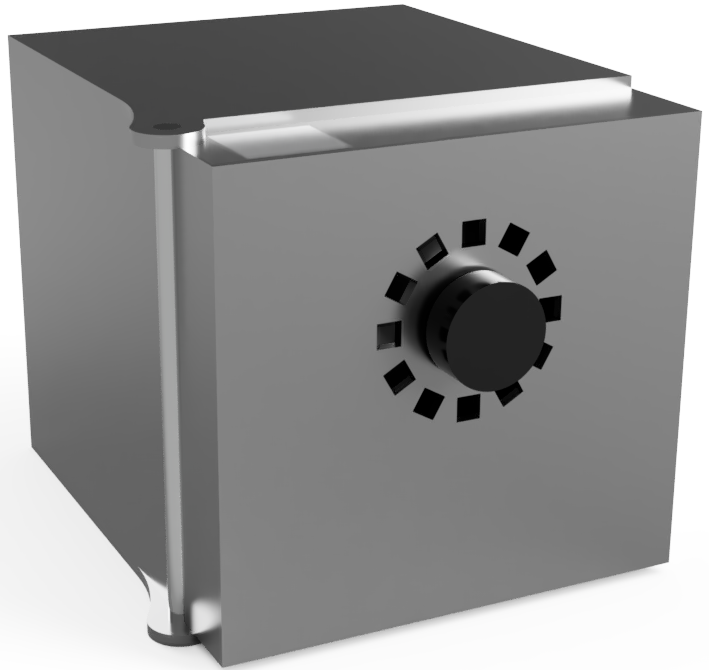
\includegraphics[width=0.5\textwidth]{kapitoly/obrazky/E2/predni_render.png}

    \appendix
    \chapter{Obrazová příloha}
	\section{Vzhled druhé elektronické varianty}
	\vspace{\OdsazeniNadpisu}
    \centering
    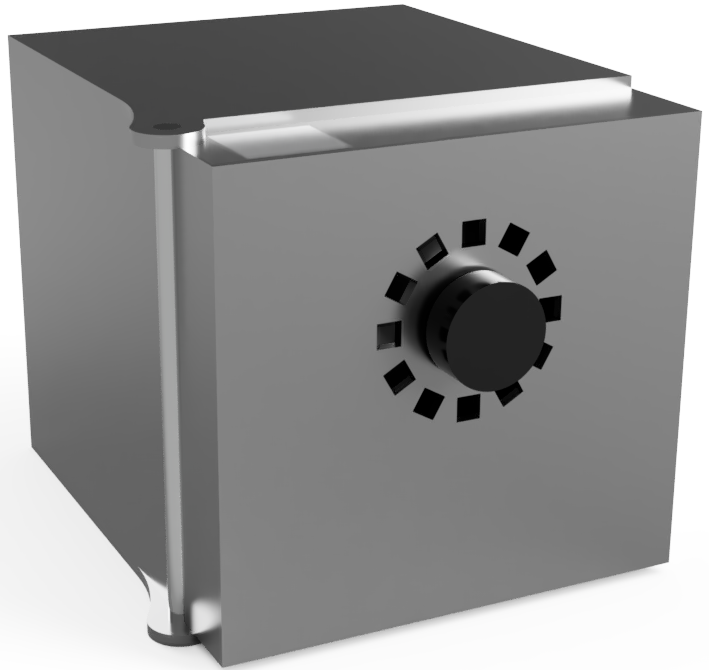
\includegraphics[width=0.7\textwidth]{kapitoly/obrazky/E2/predni_render.png}

    \caption{Render varianty E2}
    \label{fig:E2-render}
\end{figure}

\begin{figure}
    \section{Vzhled třetí elektronické varianty}
	\centering
	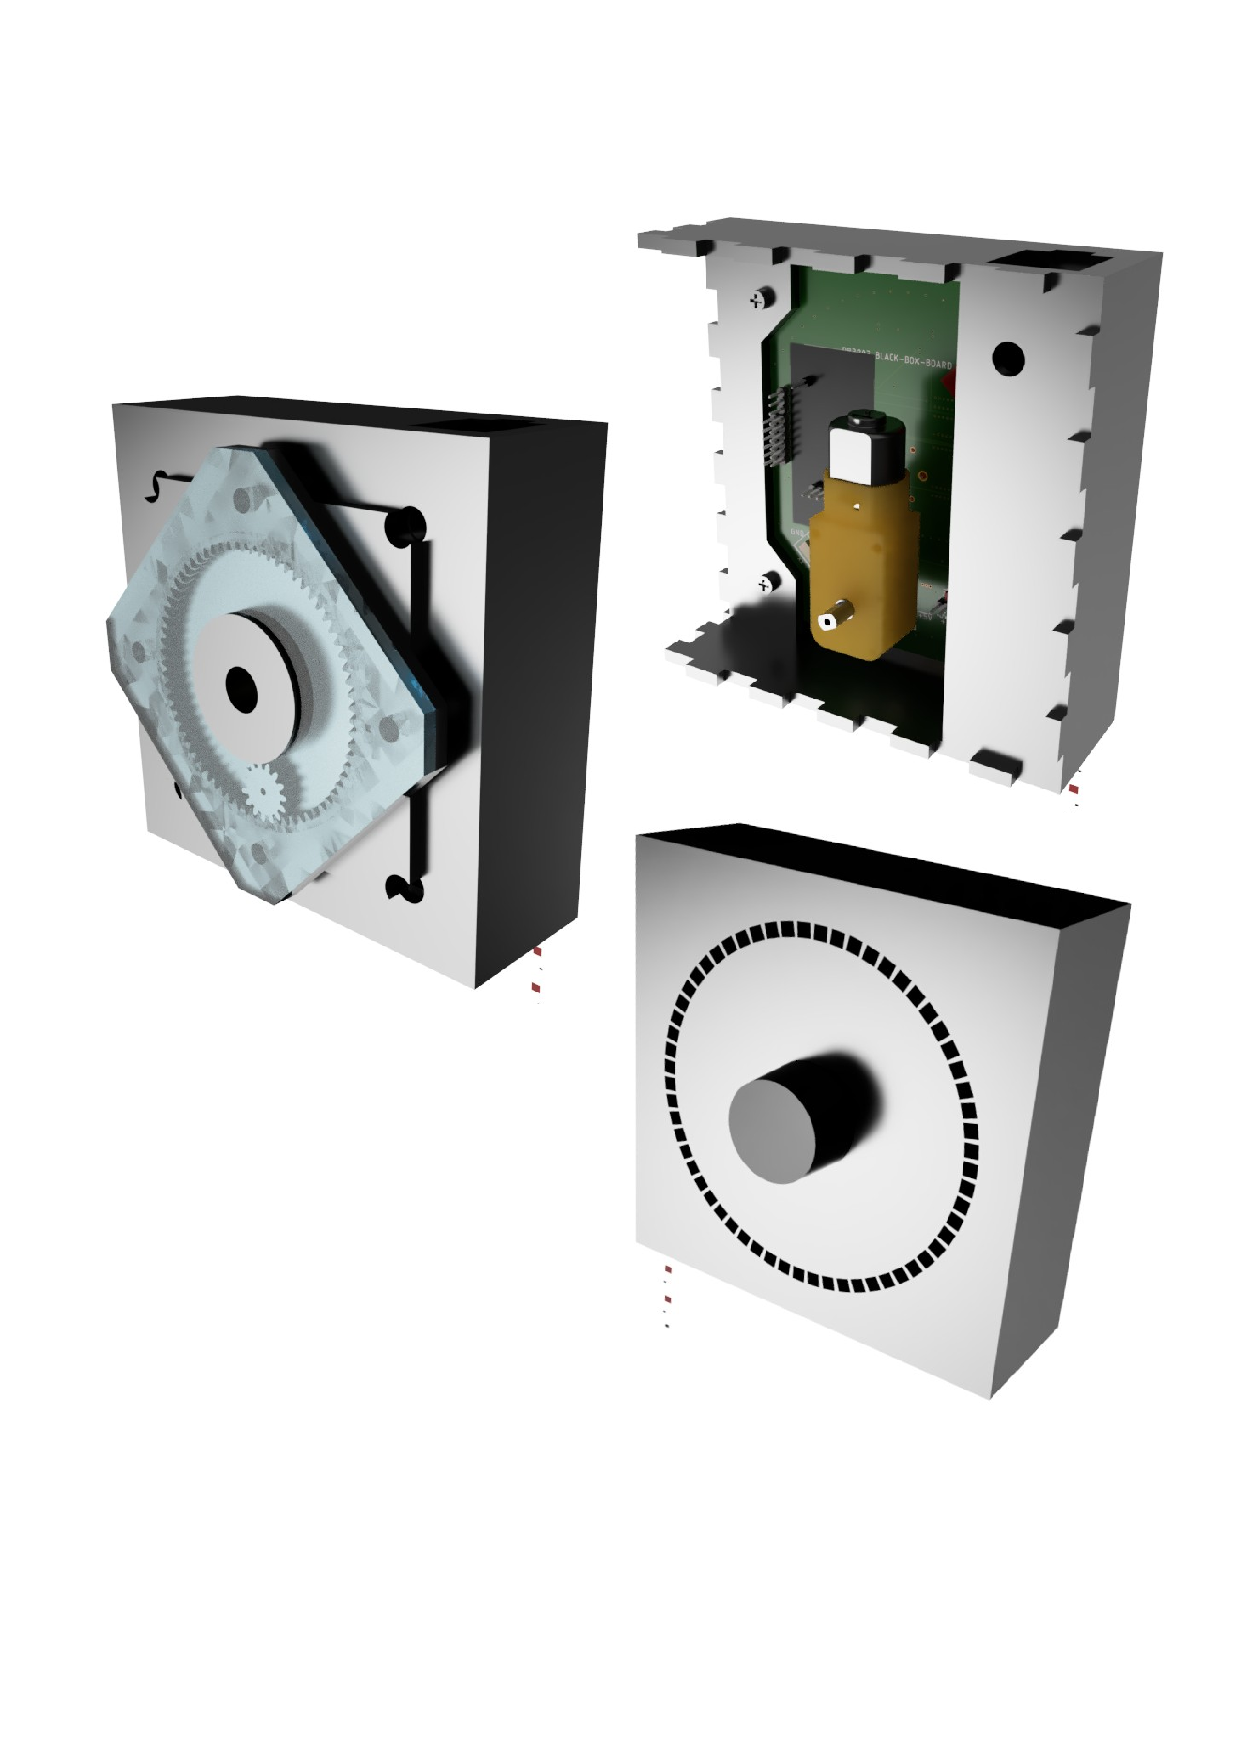
\includegraphics[width=\textwidth]{kapitoly/obrazky/E3/rendery.pdf}
	\caption{Render varianty E3}
	\label{fig:E3-renderi}
\end{figure}

\begin{figure}
	\section{Vzhled druhé mechanické varianty}
	\vspace{\OdsazeniNadpisu}
    \centering
    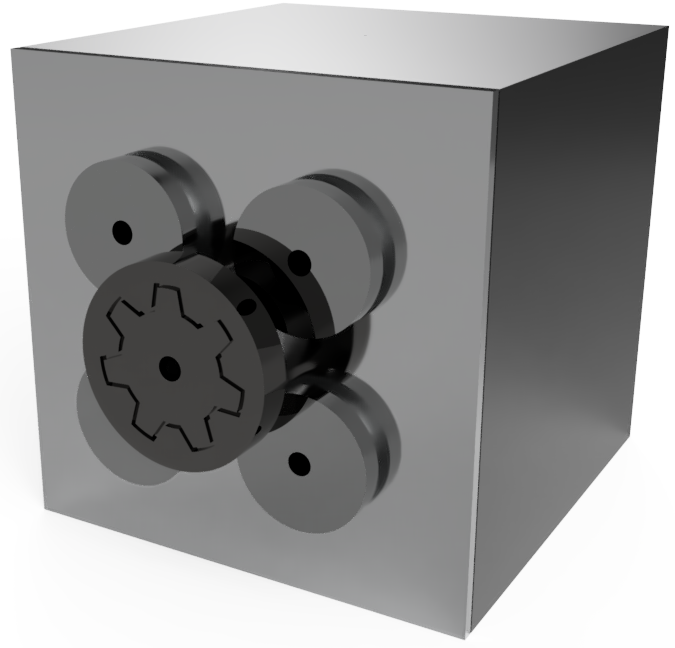
\includegraphics[width=\textwidth]{kapitoly/obrazky/M2/predni_render.PNG}
    \caption{Render varianty M2}
    \label{fig:M2-render}
\end{figure}



\begin{figure}
\section{Simulace pevnosti tlakové desky}
    %\vspace{\OdsazeniNadpisu}
    \centering
    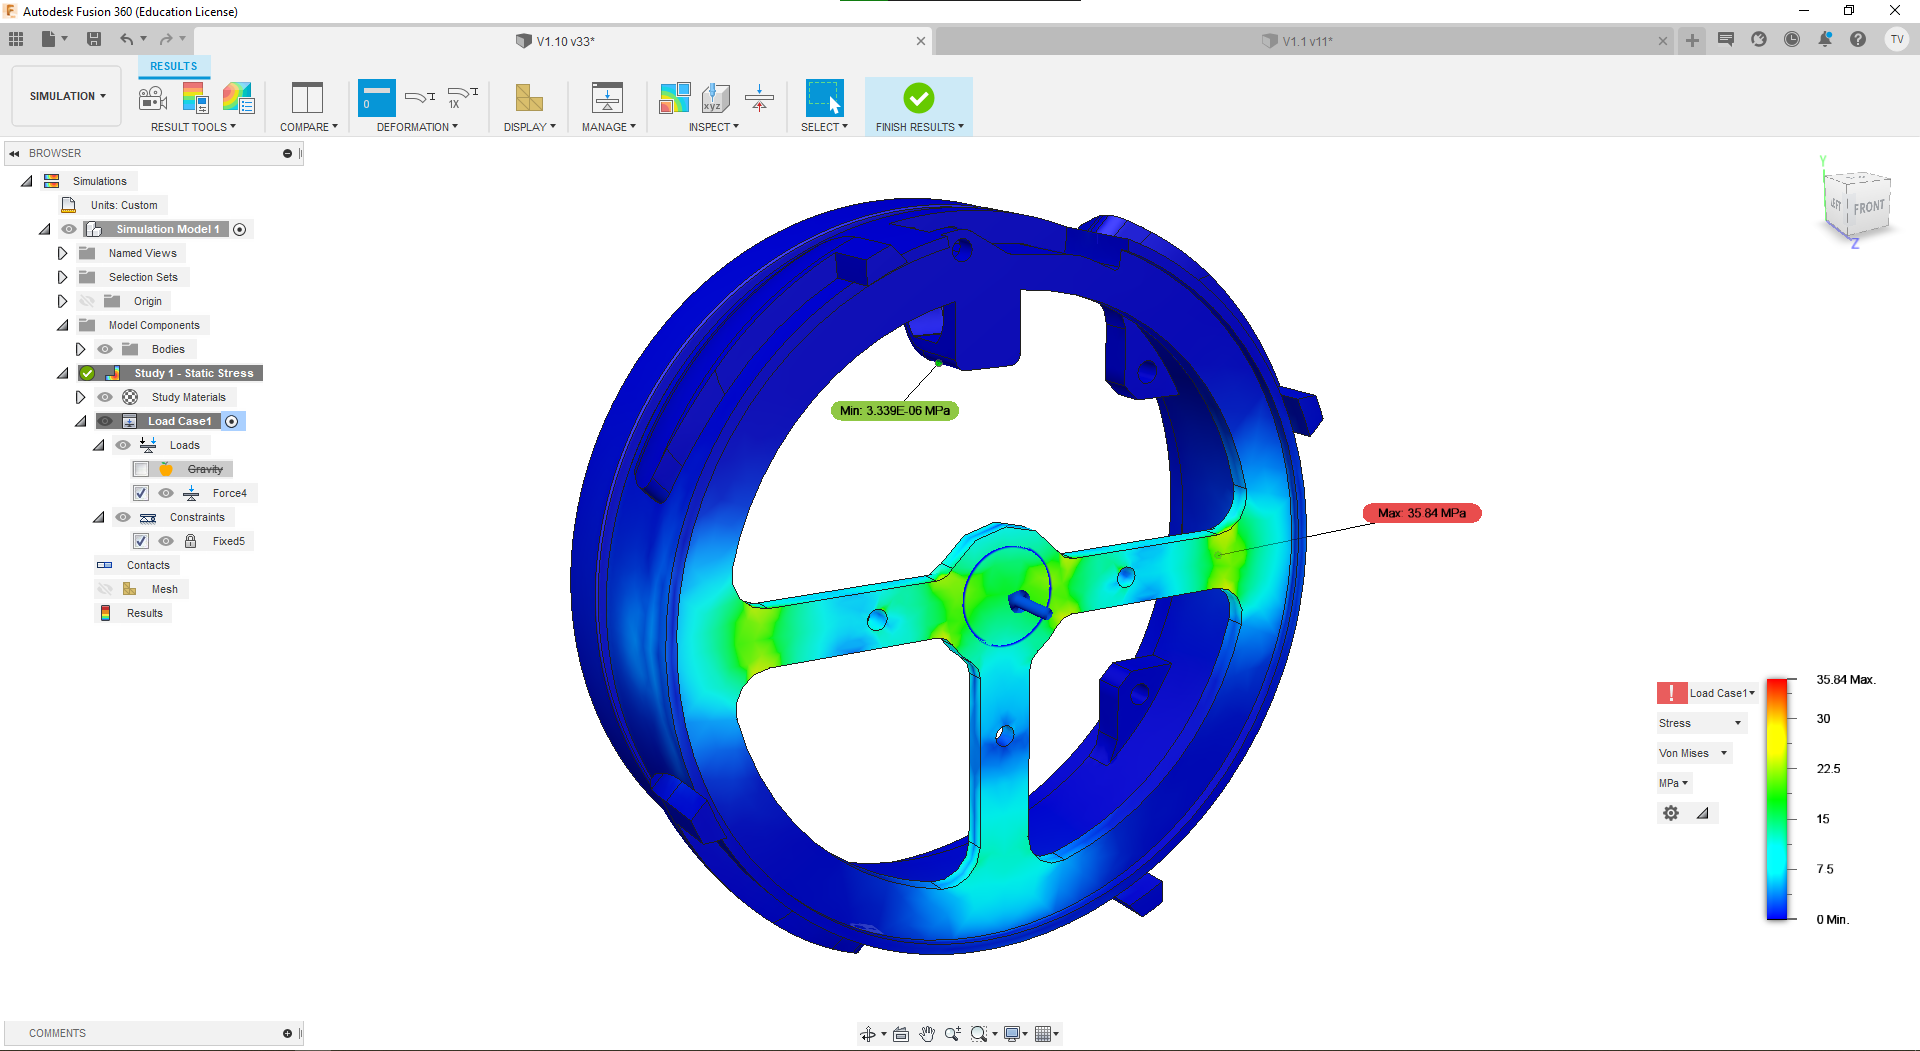
\includegraphics[width=370pt]{kapitoly/obrazky/E4/machanika_tlakove_desky/simulace/F100N,primo,uprostred,pohled_zepredu.png}
    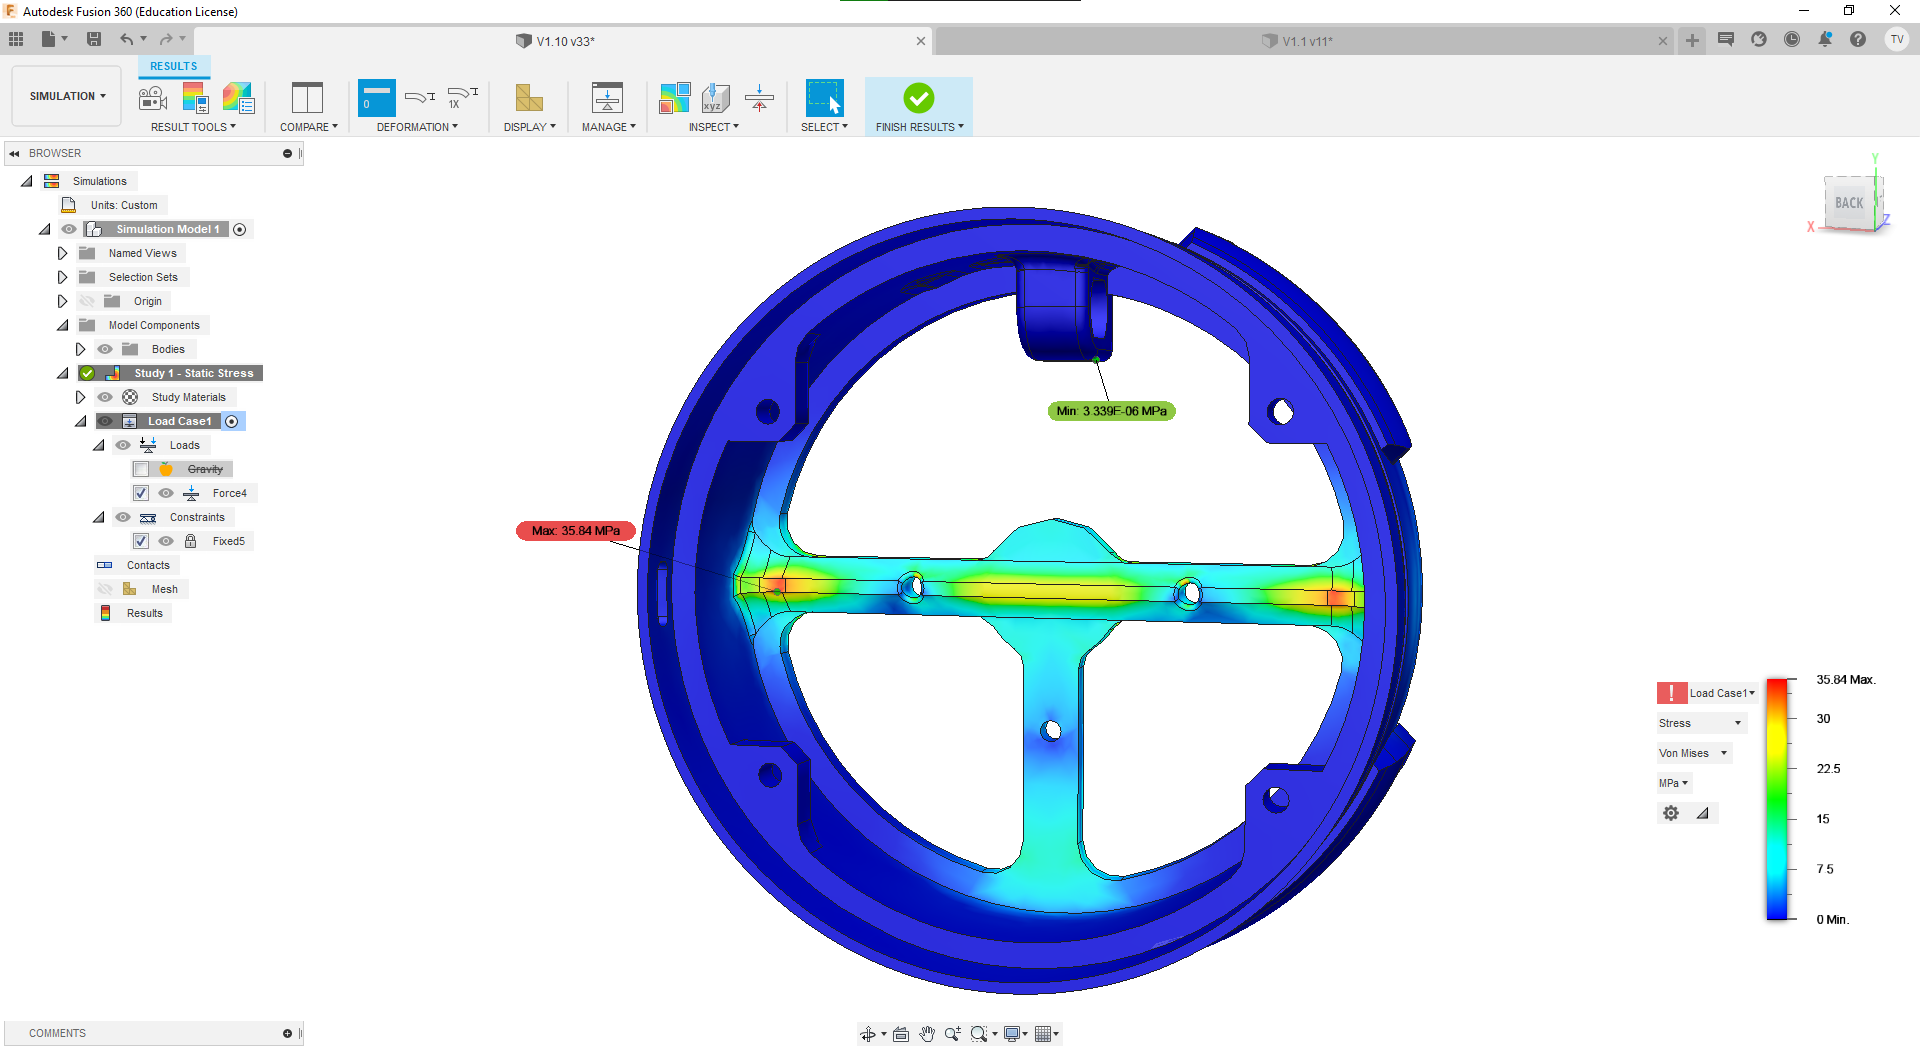
\includegraphics[width=370pt]{kapitoly/obrazky/E4/machanika_tlakove_desky/simulace/F100N,primo,uprostred,pohled_zezadu.png}
    \caption{Pevnostní simulace těla, nahoře je pohled zepředu a dole pohled zezadu \centering}
    Tato simulace testuje působení síly přímo na tělo, což není působení, které by v provozu nastávalo. Takovéto namáhání je ale o dost náročnější
    než to, které by reálně nastalo.
    \label{fig:E4-simulace_tela} %todo těla čeho? trezor je hranatý? 
\end{figure}

\begin{figure}
    \centering
    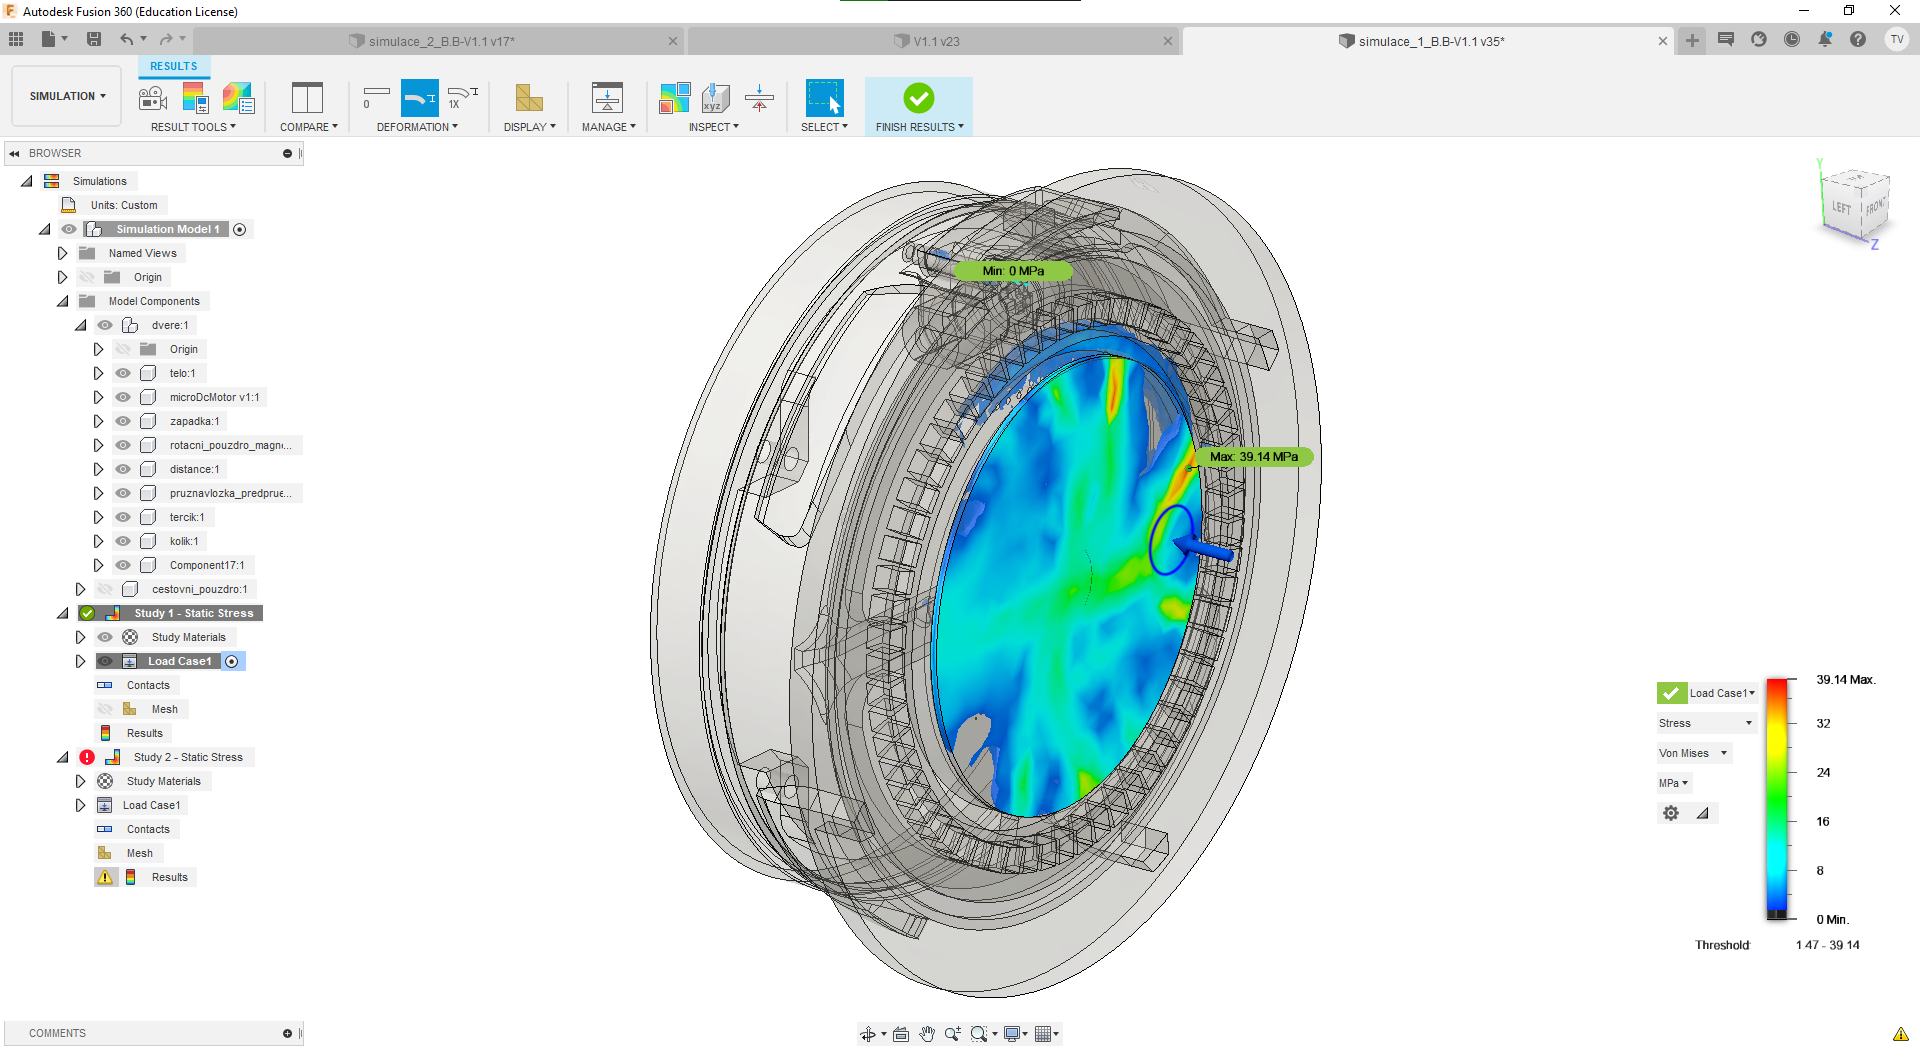
\includegraphics[width=\textwidth]{kapitoly/obrazky/E4/machanika_tlakove_desky/simulace/zjednodusena_sestava_pri_F100N_nezobrazeno_napeti_pod_1,5MPa.png}
    \caption{Simulace sestavy}
    Jak je vidět, tak i sílu 100~N dokaže, sendvič z terčíku, pružné podložky a~snímací desky rozložit na dostatečnou plochu, aby napětí v těle nestouplo 
    nad cca 3~MPa. Na obrázku je zobrazené jen napětí nad 1,5~MPa.
    \label{fig:E4-simulace_tlakovky}
\end{figure}

\begin{figure}[h]
    \centering
    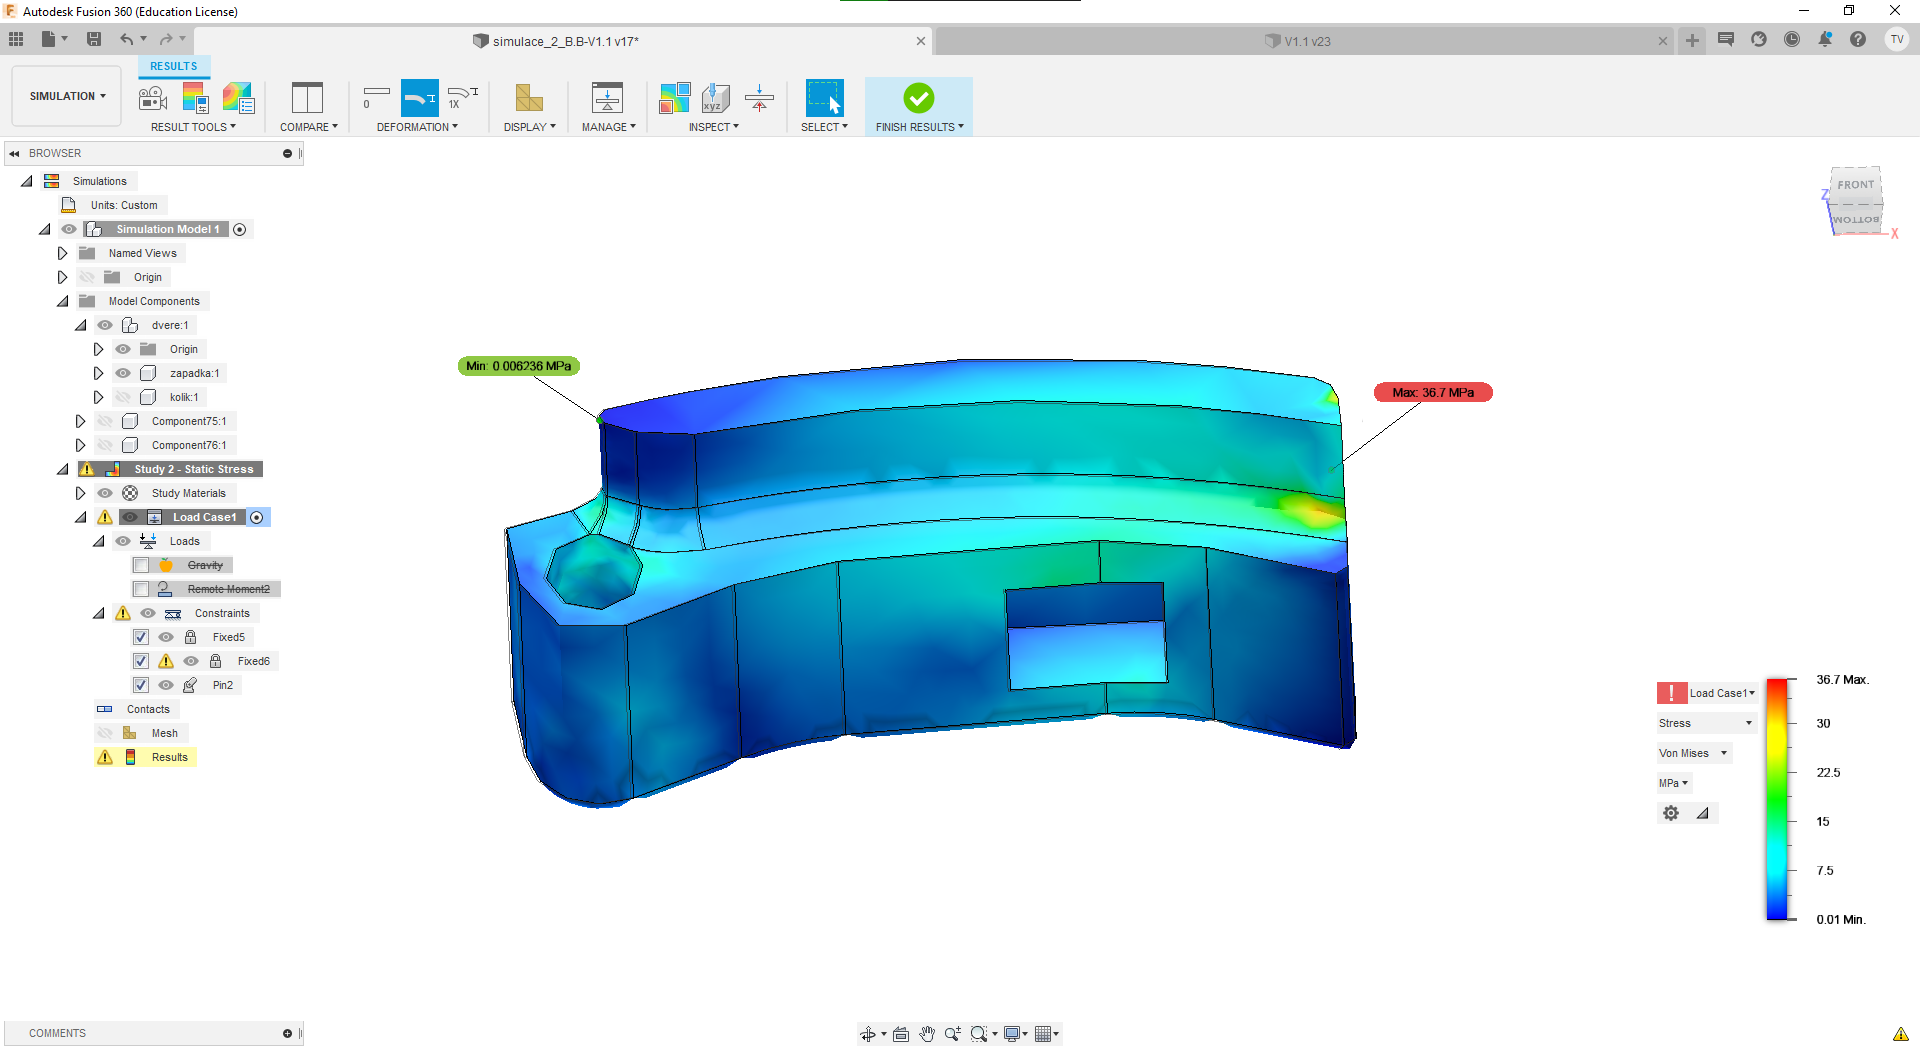
\includegraphics[width=\textwidth]{kapitoly/obrazky/E4/zapadka/simulace/napeti_D1-M5000.png}
    \caption{Simulace napětí v západce při kroutícím momentu 5000 N $\cdot$ mm což na rameni 48~mm znamená sílu působící na kolík 104~N}
    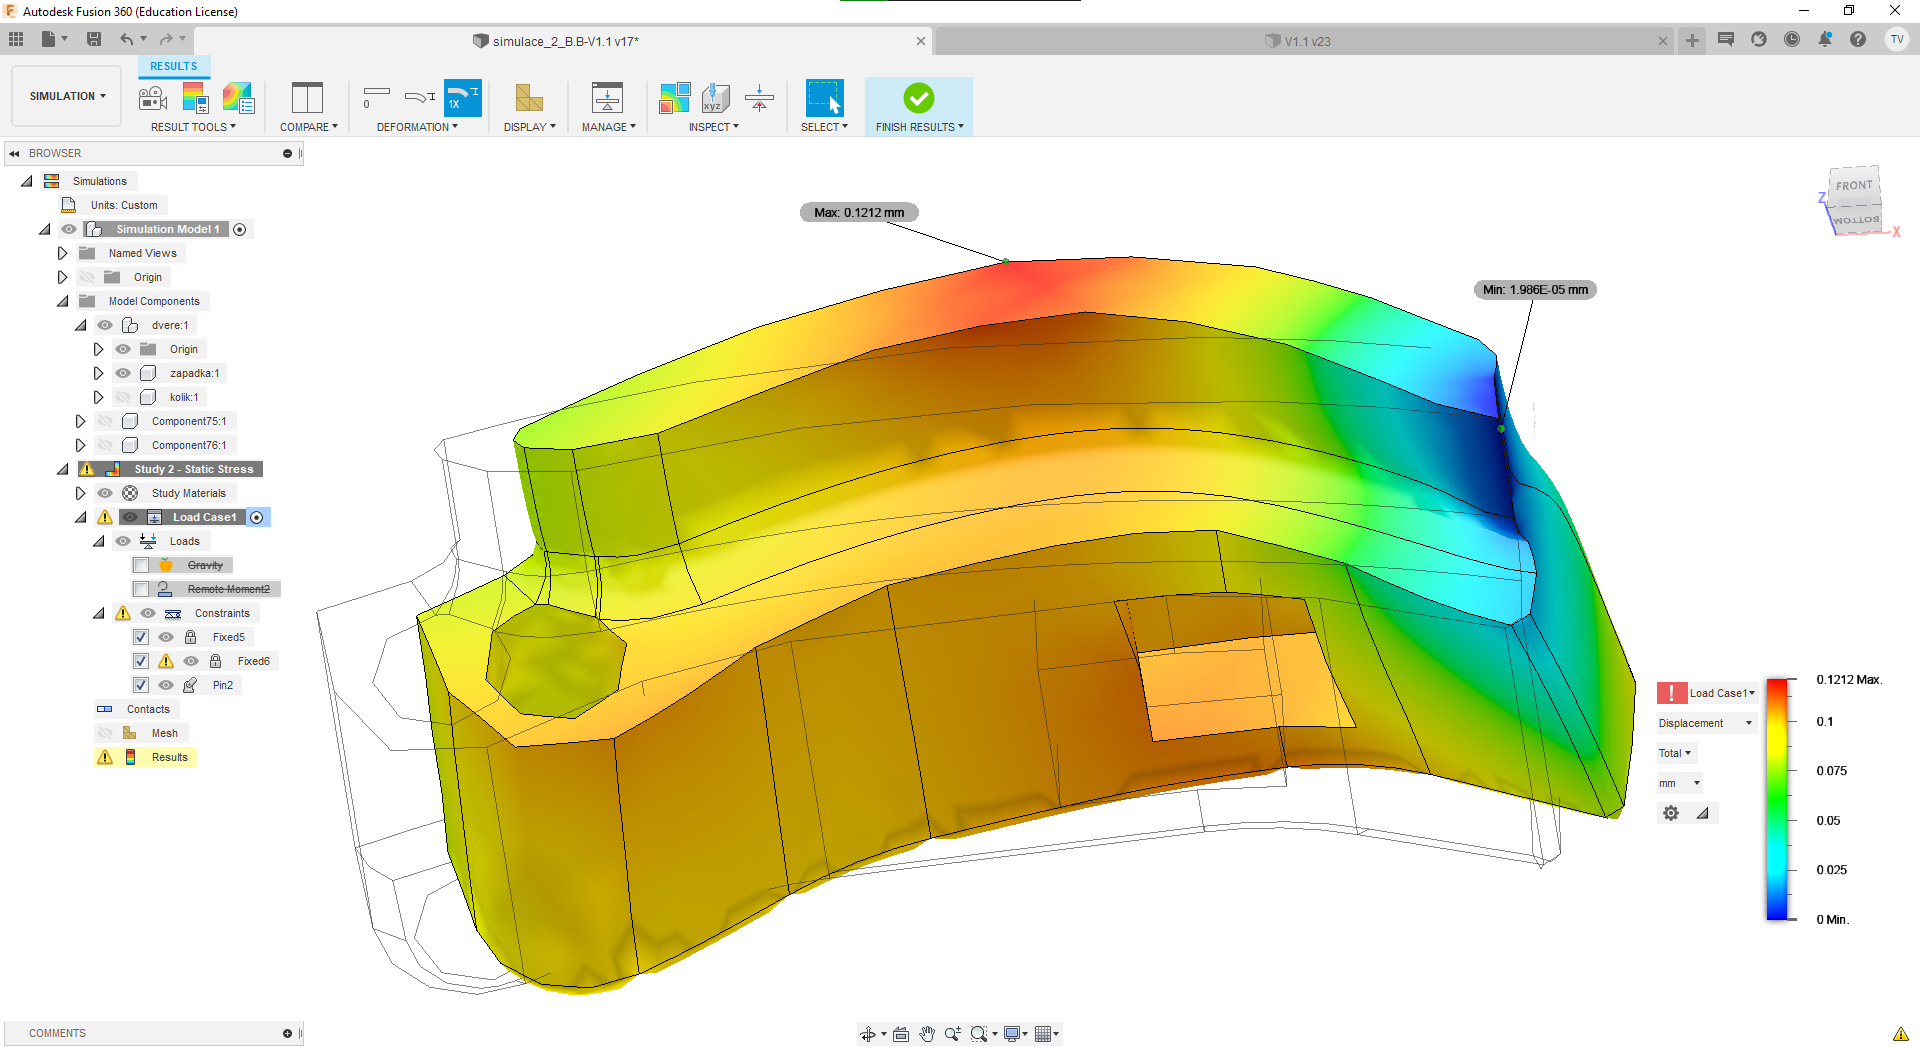
\includegraphics[width=\textwidth]{kapitoly/obrazky/E4/zapadka/simulace/Dislokace_D10-M5000.png}
    \caption{Zobrazení deformace, pro lepší zobrazení je deformace zdesetinásobená}
    \label{fig:E4-simulace_zapadky}
\end{figure}

\begin{figure}
\section{Obrázky DPS}
    %\vspace{\OdsazeniNadpisu}
    \centering
    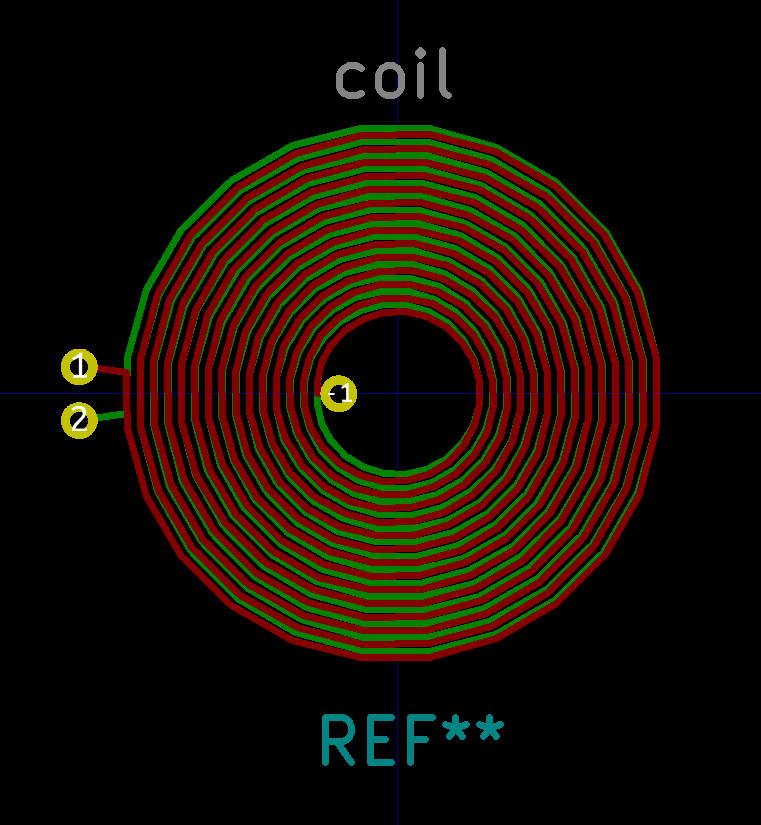
\includegraphics[width=\textwidth]{kapitoly/obrazky/E4/elektronika_tlakove_desky/civka.png}
    \caption{Vzhled reliéfu cívky}
    \label{fig:E4-relief_civka}
\end{figure}

\begin{figure}
    \centering
    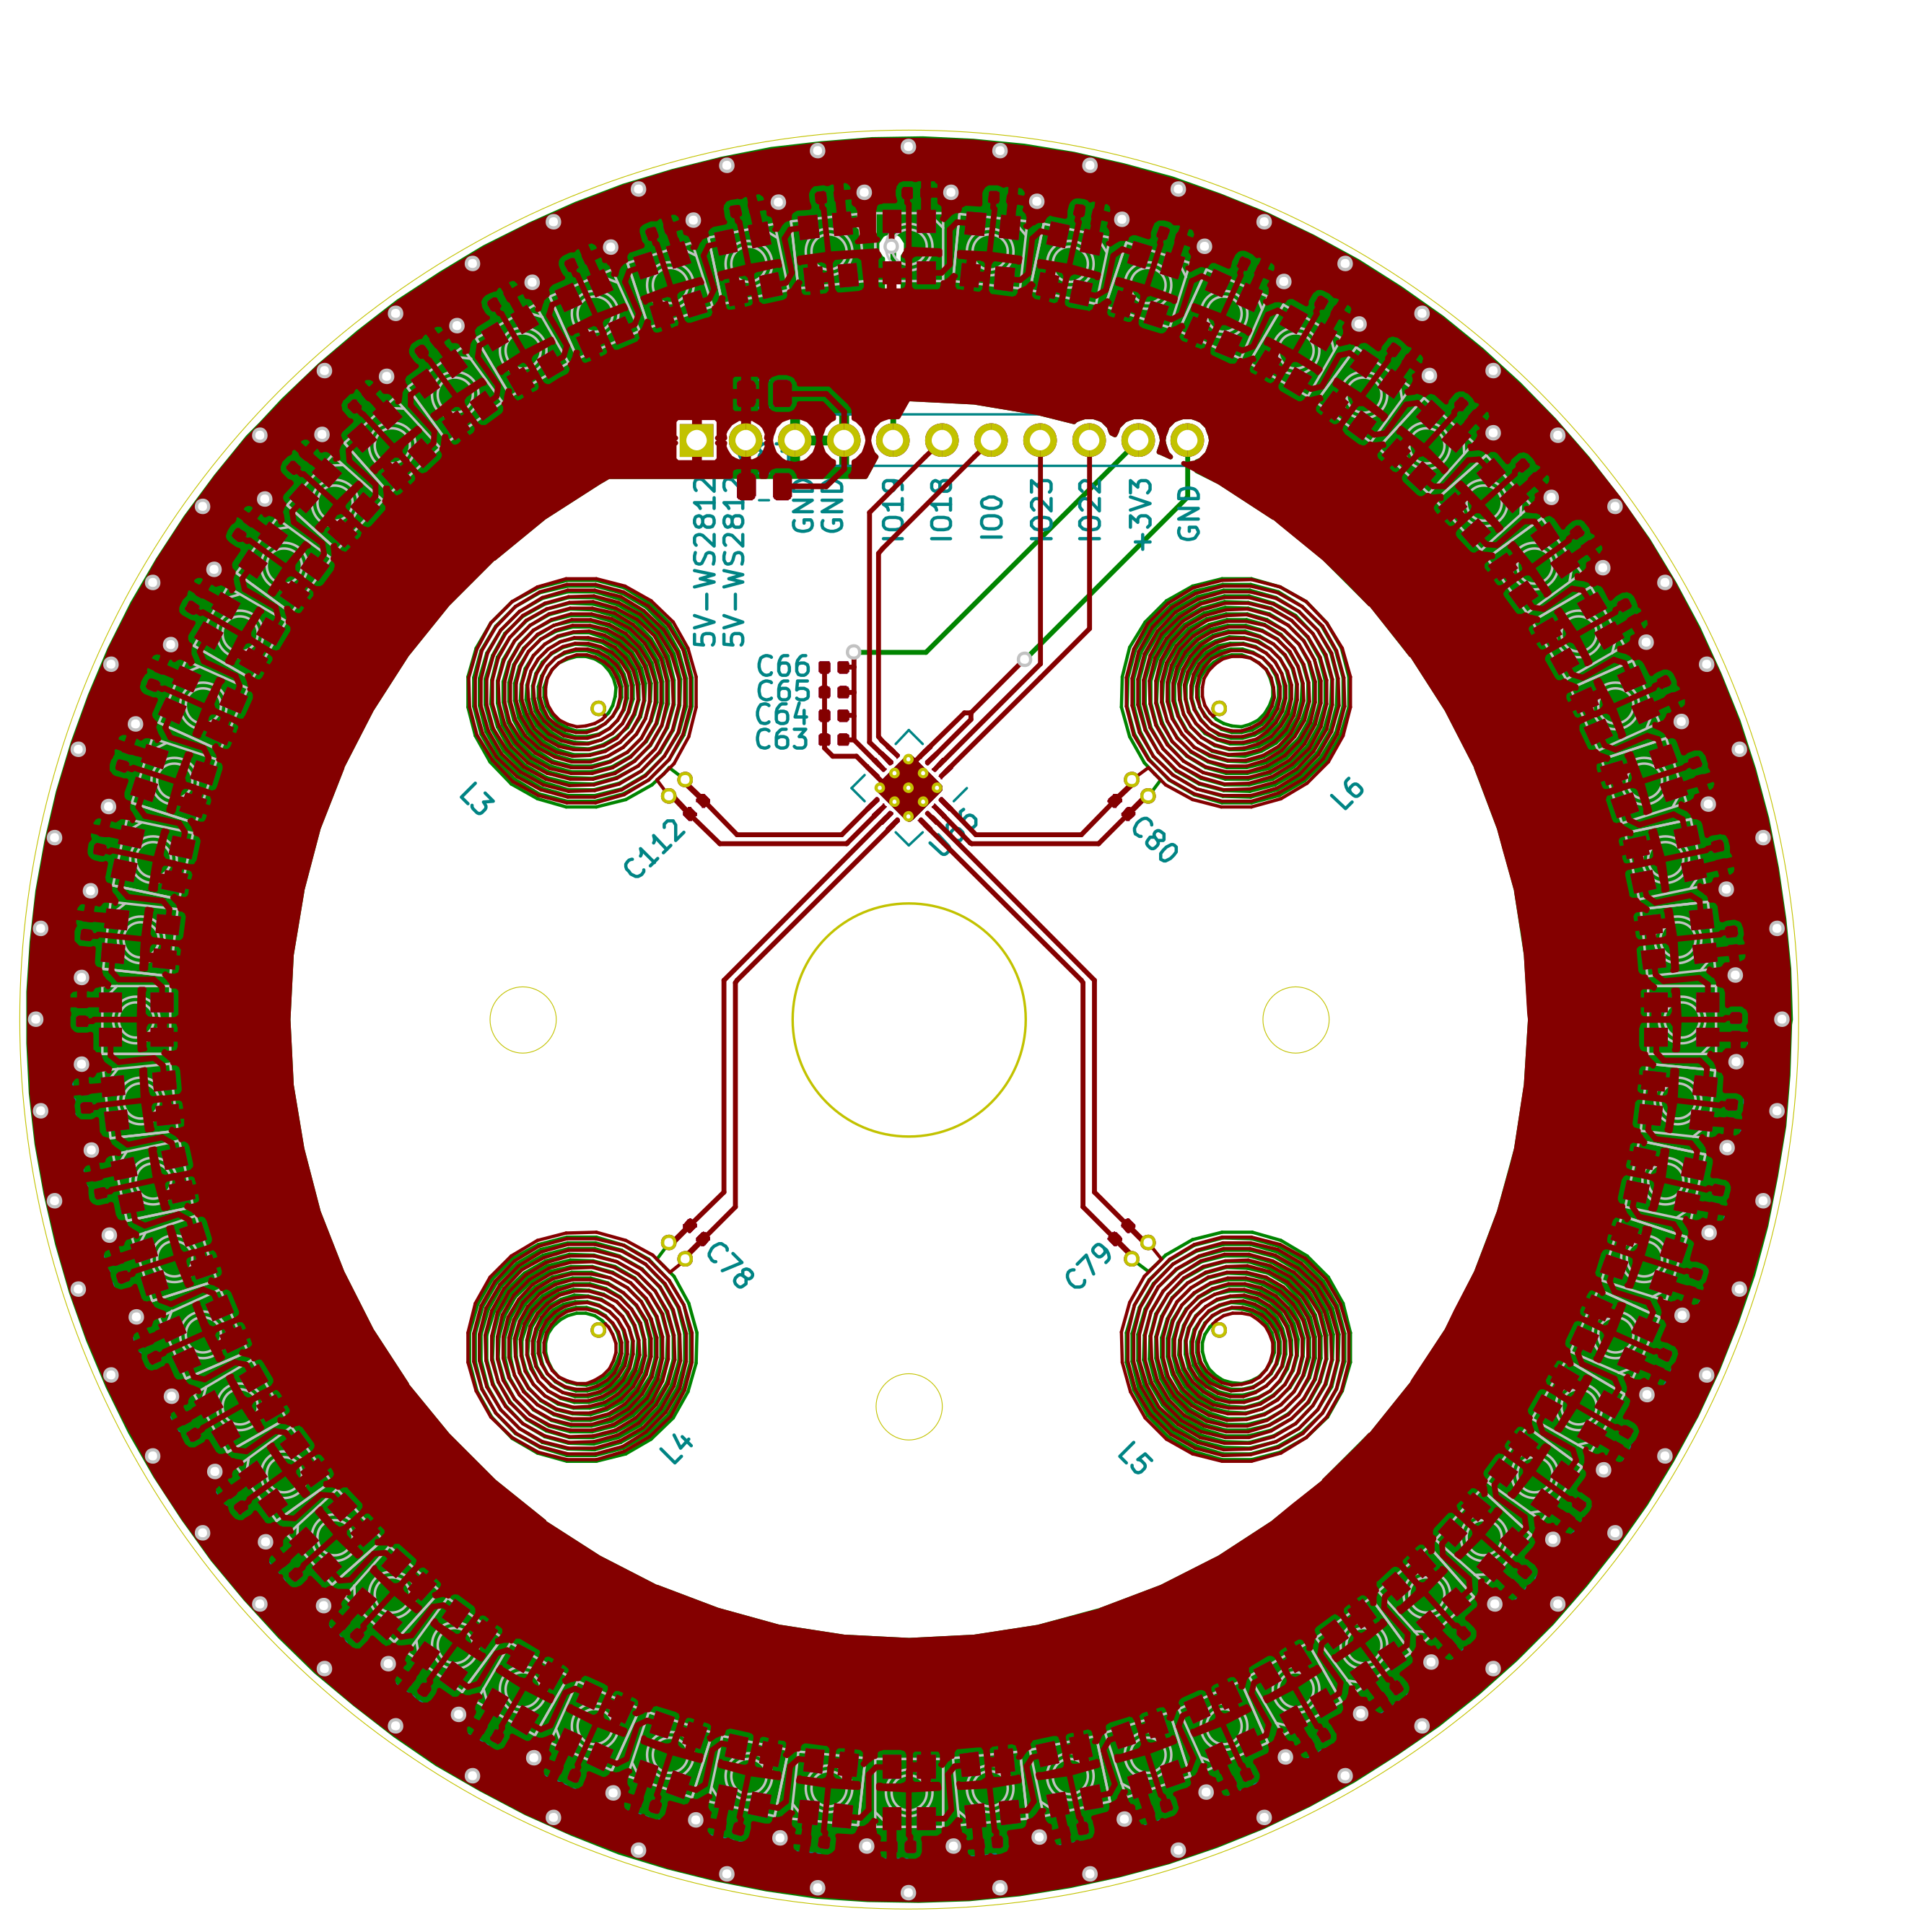
\includegraphics[width=\textwidth]{kapitoly/obrazky/E4/E4-LEDBoard.png}
    \caption{Vzhled desky s kruhem WS2812 a snímáním tlakové desky}
    \label{fig:E4-LedDeska}
\end{figure}

\begin{figure}
    \centering
    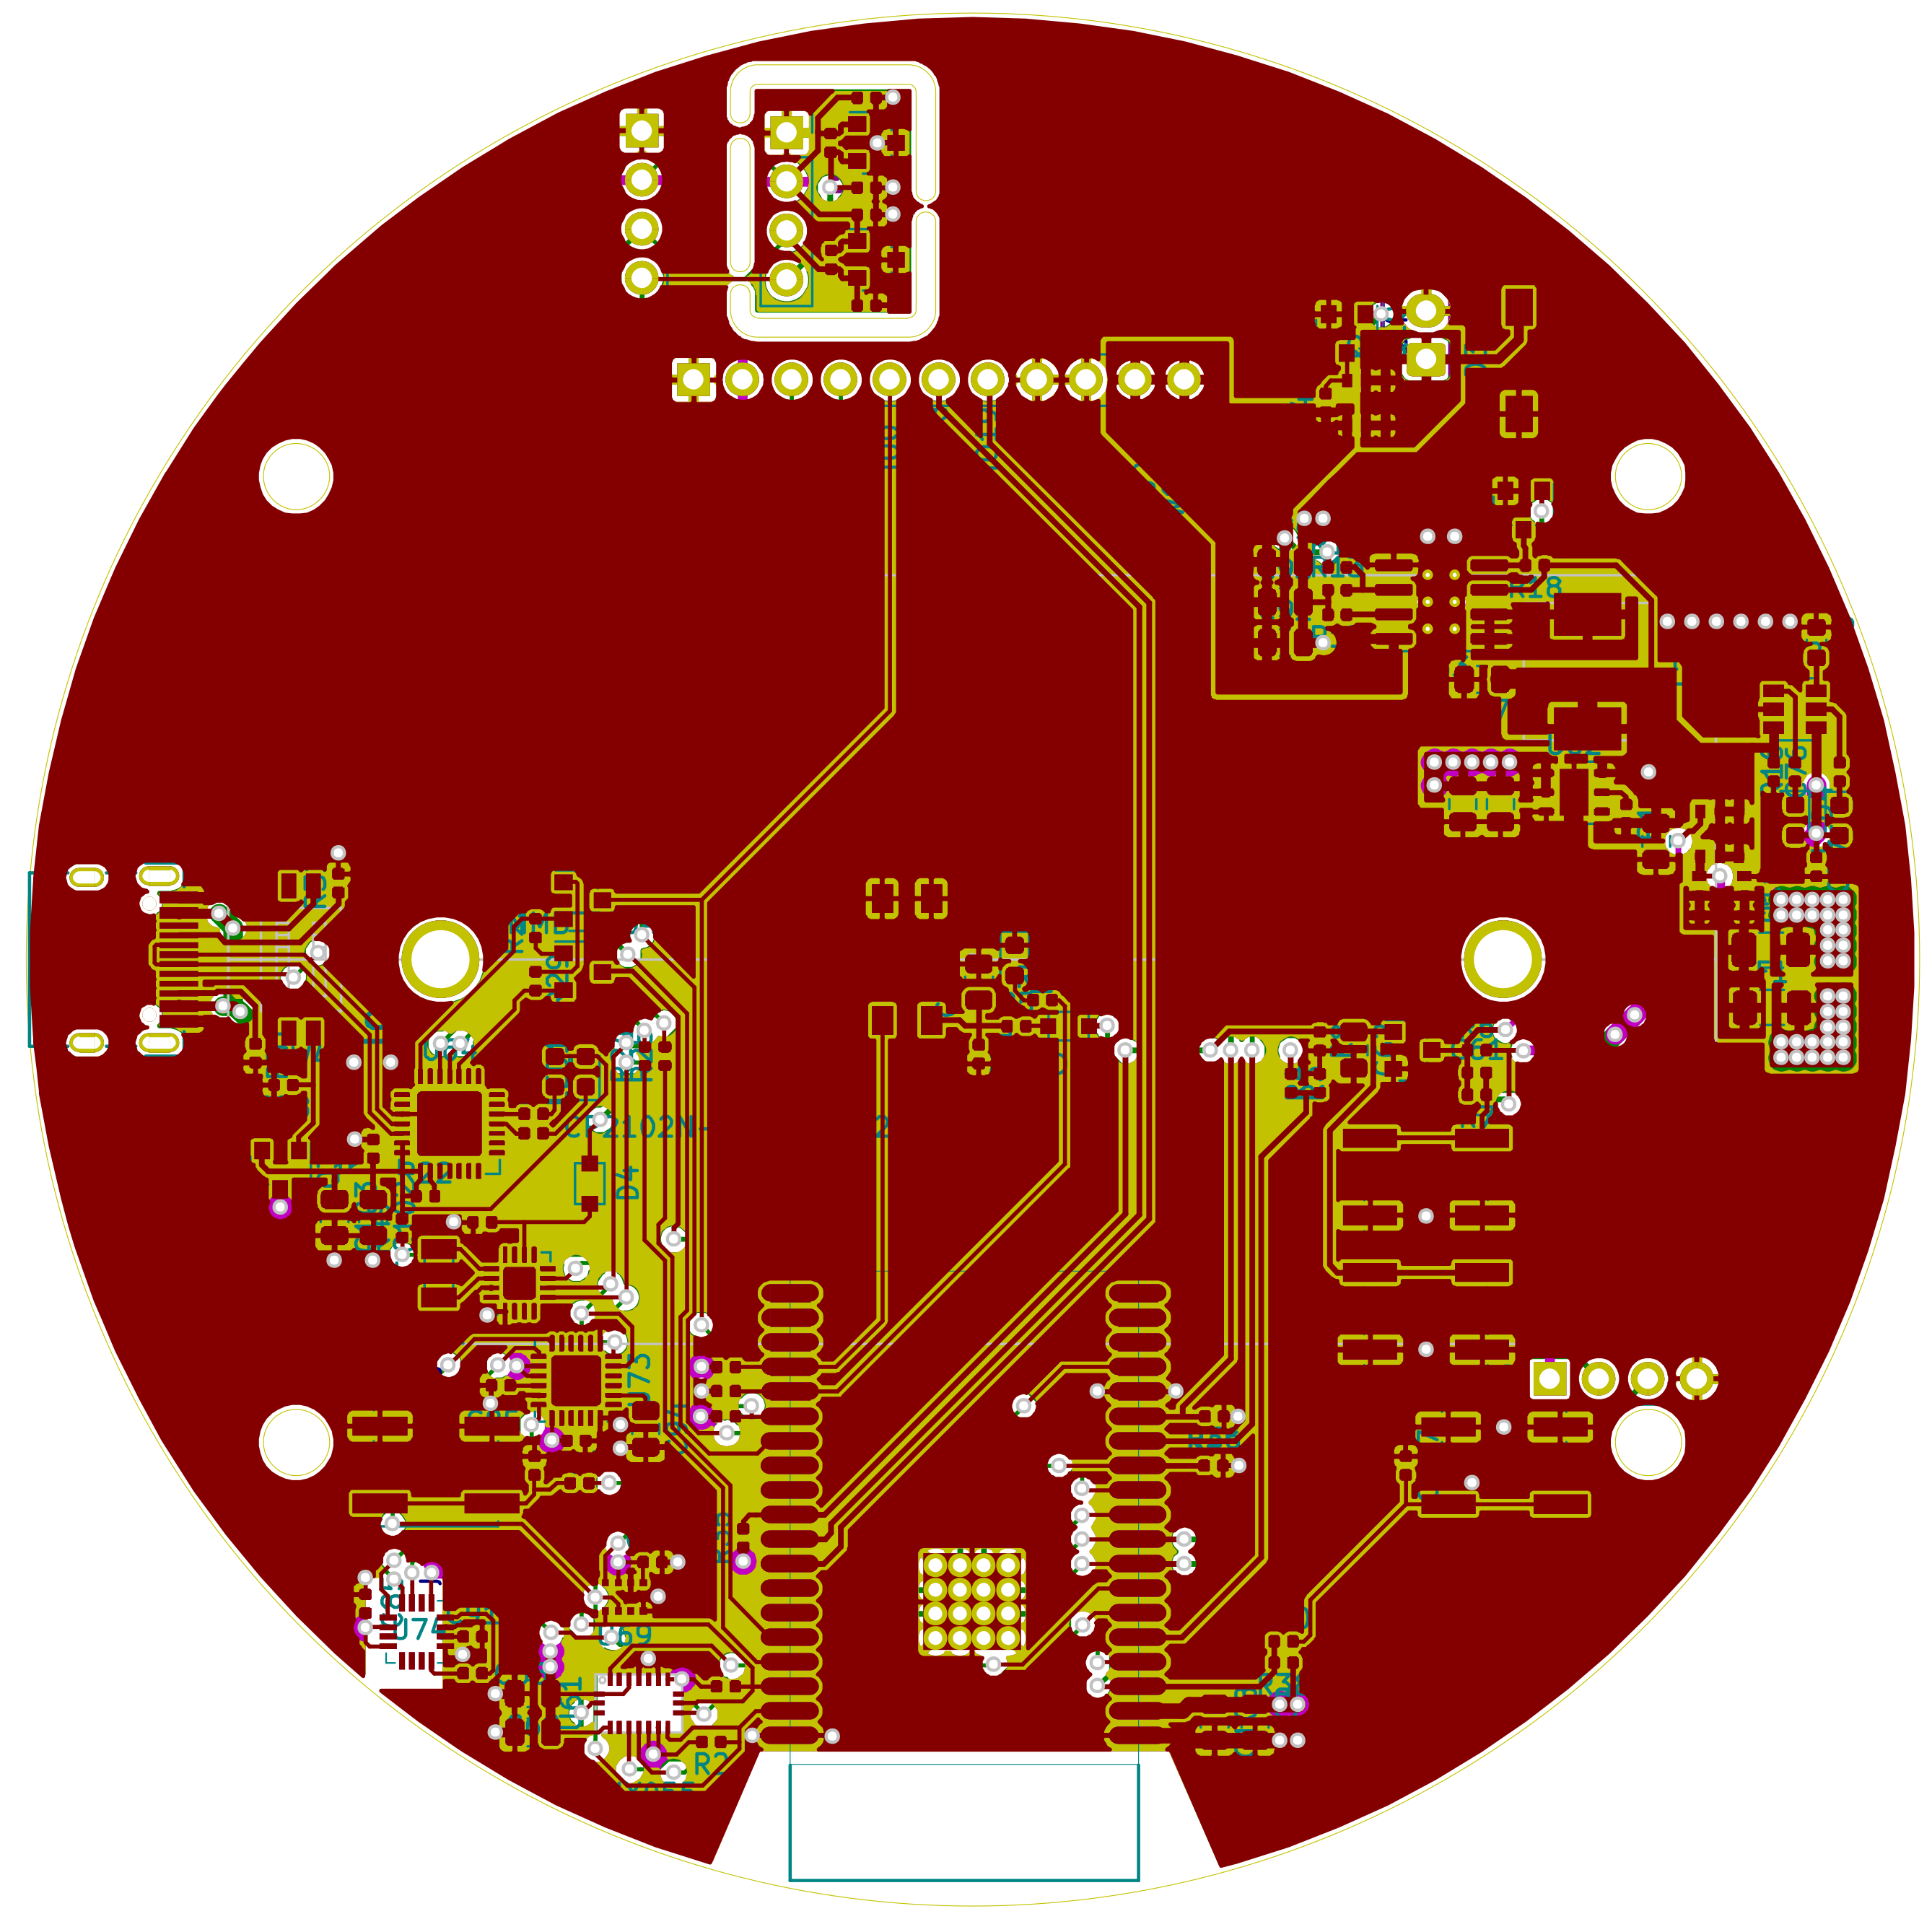
\includegraphics[width=\textwidth]{kapitoly/obrazky/E4/E4-MainBoard.png}
    \caption{Vzhled hlavní desky}
    \label{fig:E4-MainBoard}
\end{figure}



\begin{figure}
	\section{Schémata}
    \centering
    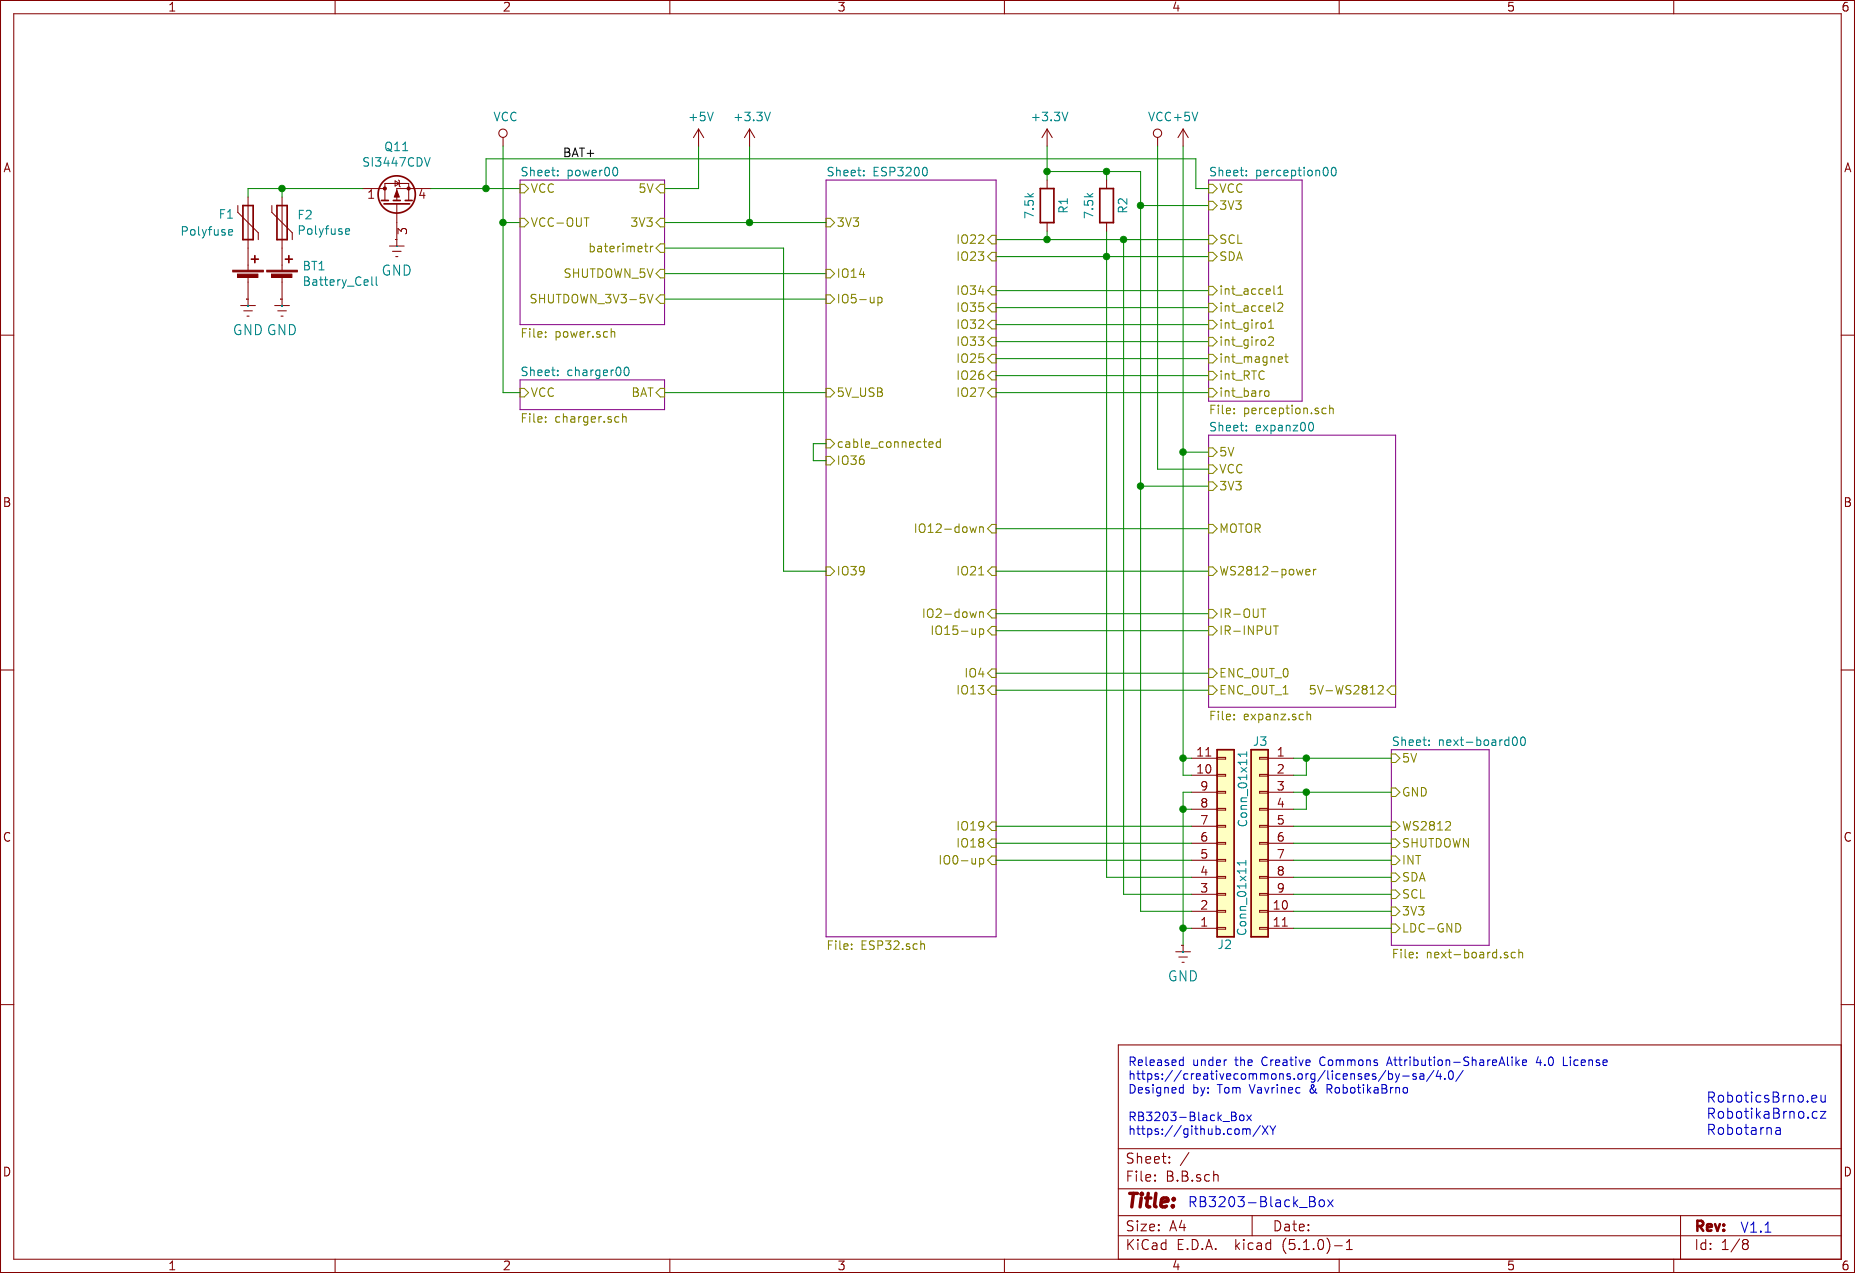
\includegraphics[width=0.93\textheight, angle=90]{kapitoly/ctvrta_elektronicka_varianta/E4_zapojeni/B.B.png}
    \caption{Propojení jednotlivých systémů -- schéma}
    \label{fig:E4-sch_B.B}
\end{figure}
\begin{figure}
    \centering
    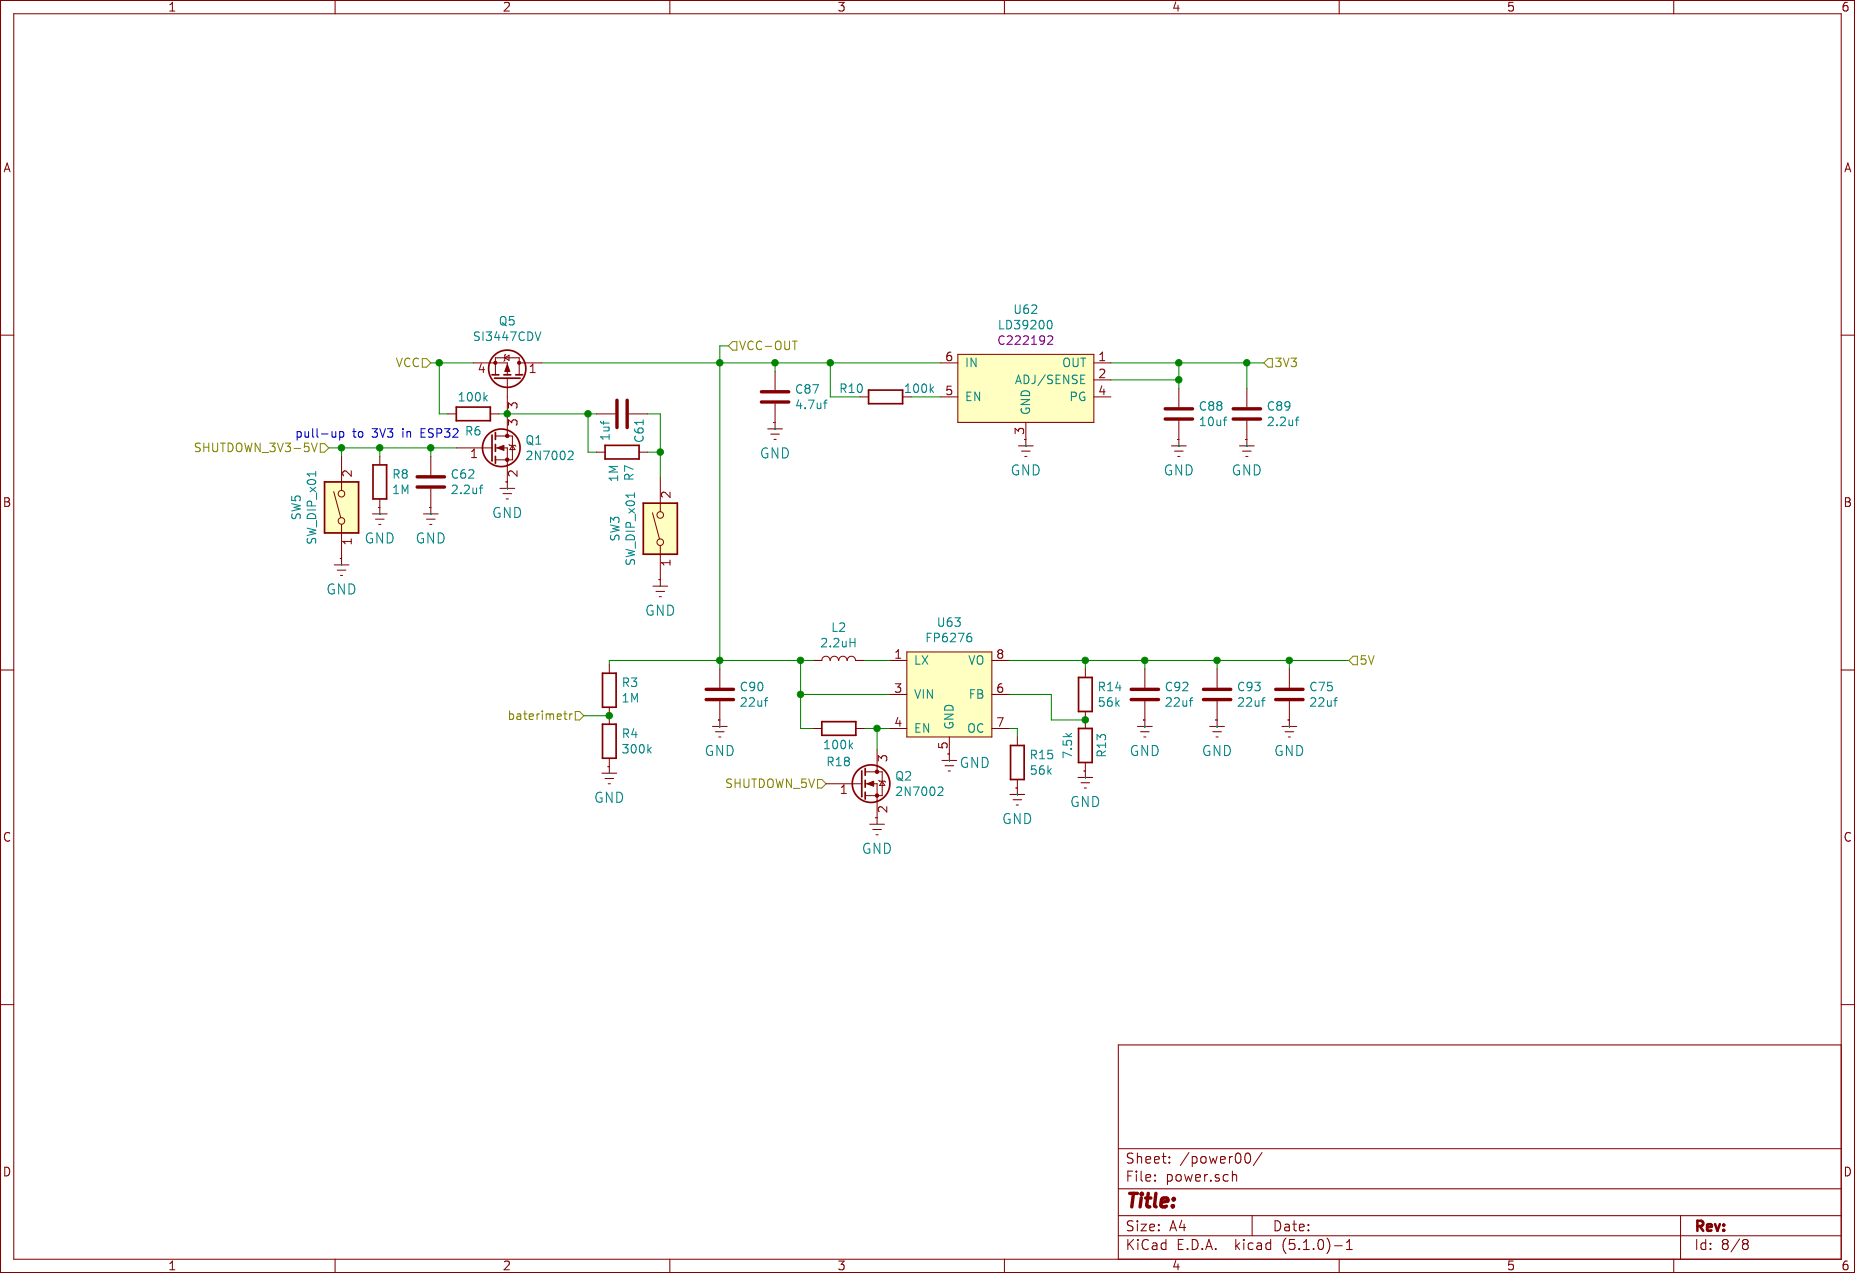
\includegraphics[width=0.93\textheight, angle=90]{kapitoly/ctvrta_elektronicka_varianta/E4_zapojeni/zdroj.png}
    \caption{Zapojení zdroje -- schéma}
    \label{fig:E4-sch_zdroj}
\end{figure}
\begin{figure}
    \centering
    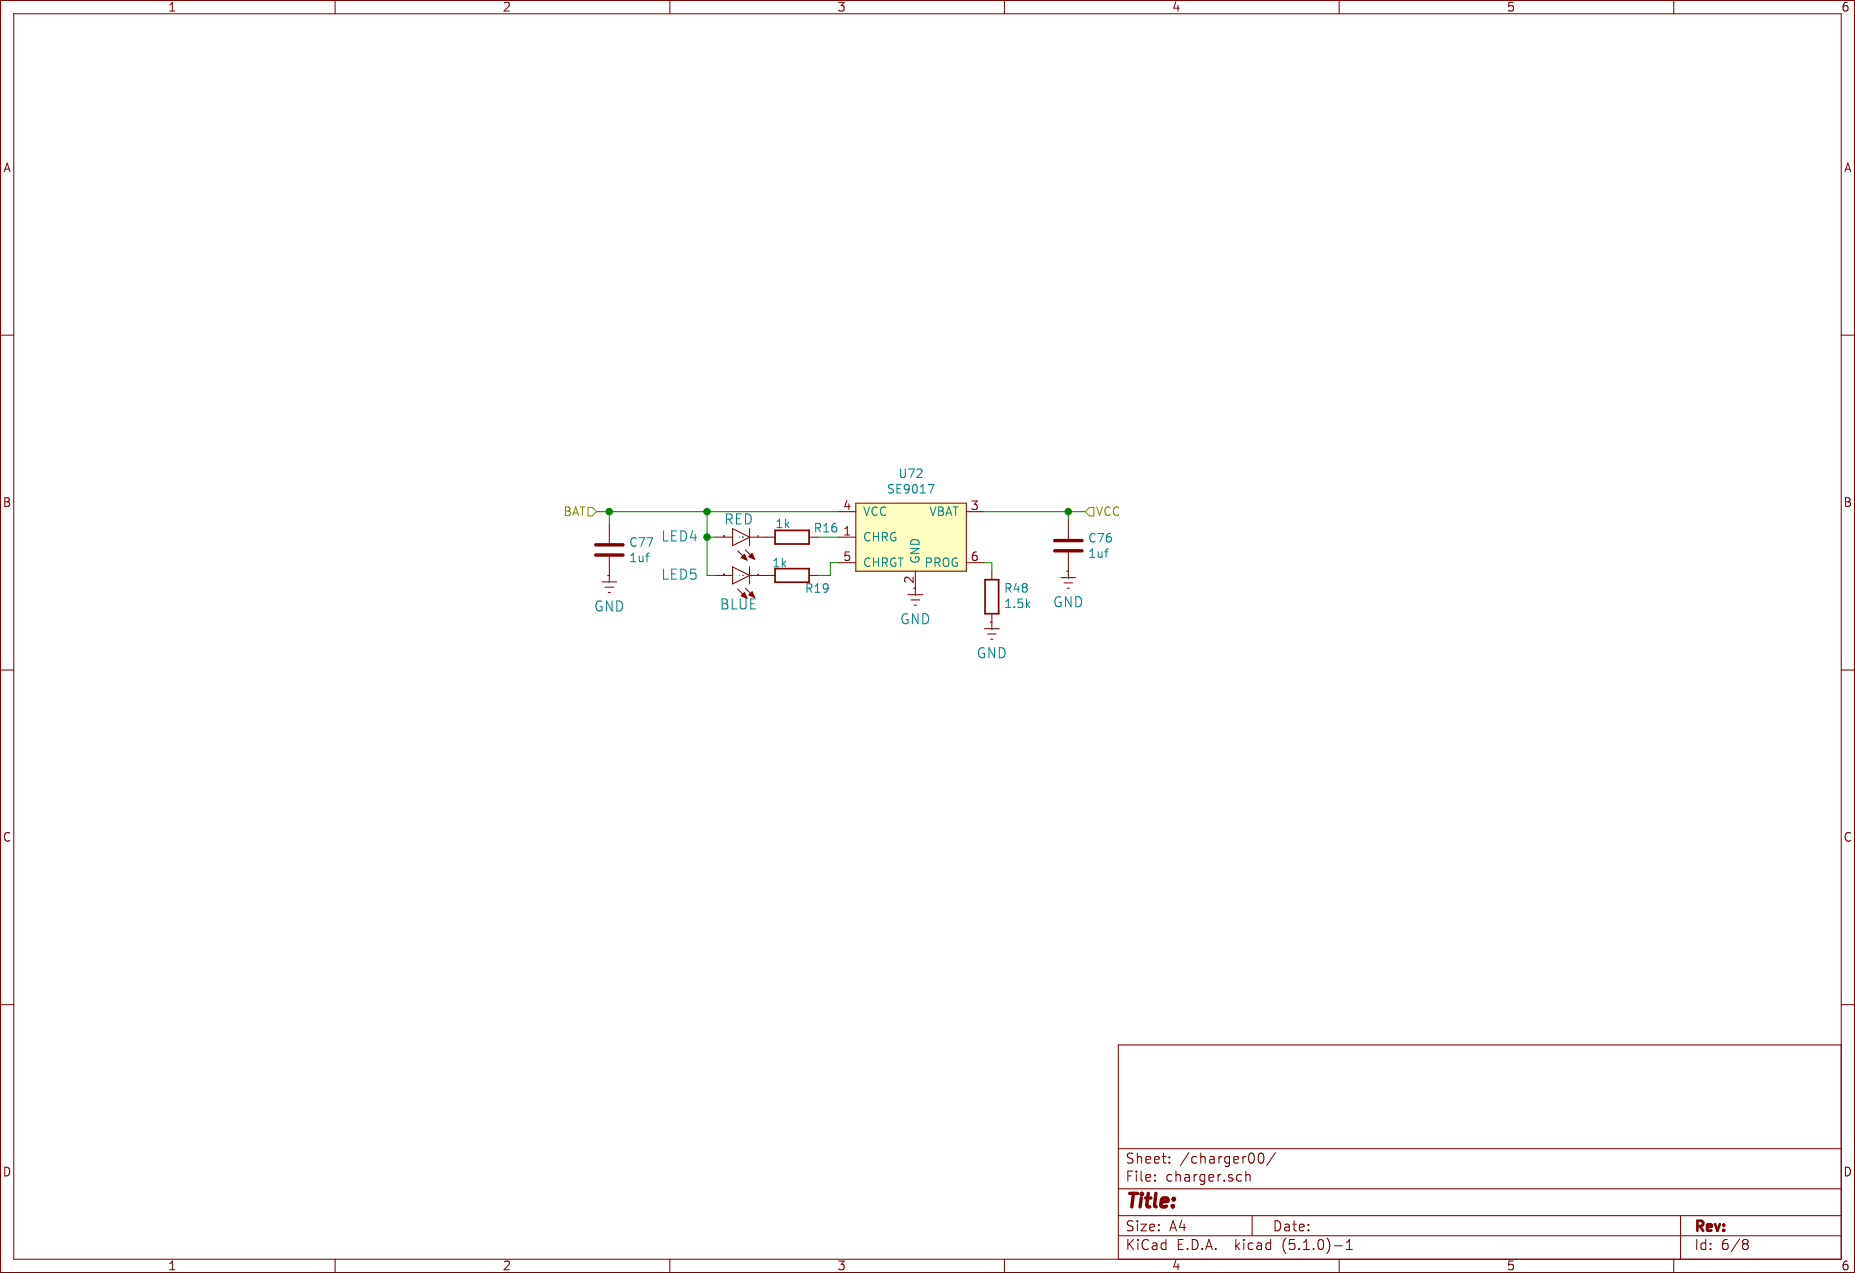
\includegraphics[width=0.93\textheight, angle=90]{kapitoly/ctvrta_elektronicka_varianta/E4_zapojeni/nabijecka.png}
    \caption{Zapojení nabíjecího obvodu -- schéma}
    \label{fig:E4-sch_nabijecka}
\end{figure}
\begin{figure}
    \centering
    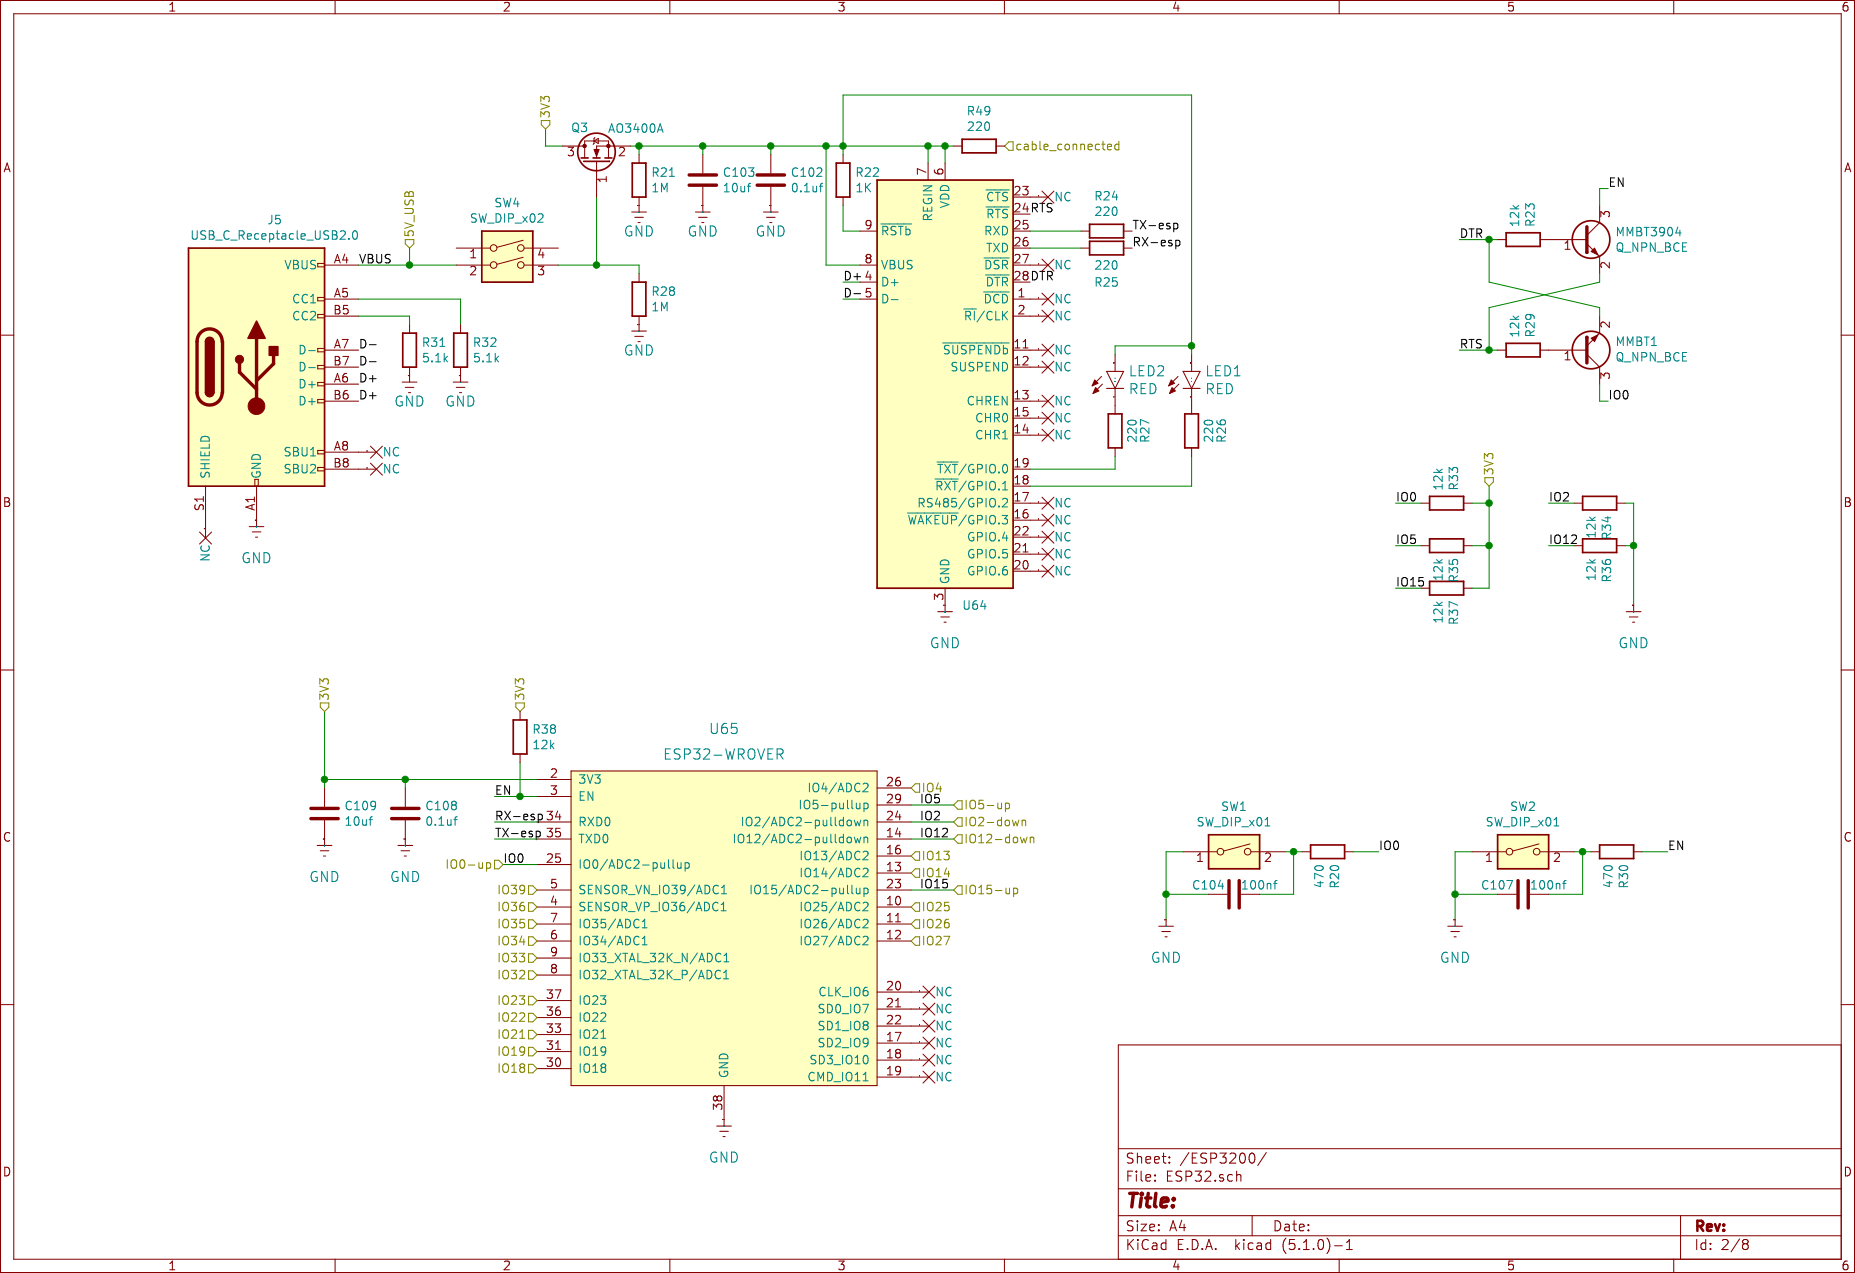
\includegraphics[width=0.93\textheight, angle=90]{kapitoly/ctvrta_elektronicka_varianta/E4_zapojeni/ESP32.png}
    \caption{Zapojení ESP32 a programátoru -- schéma}
    \label{fig:E4-sch_ESP32}
\end{figure}
\begin{figure}
    \centering
    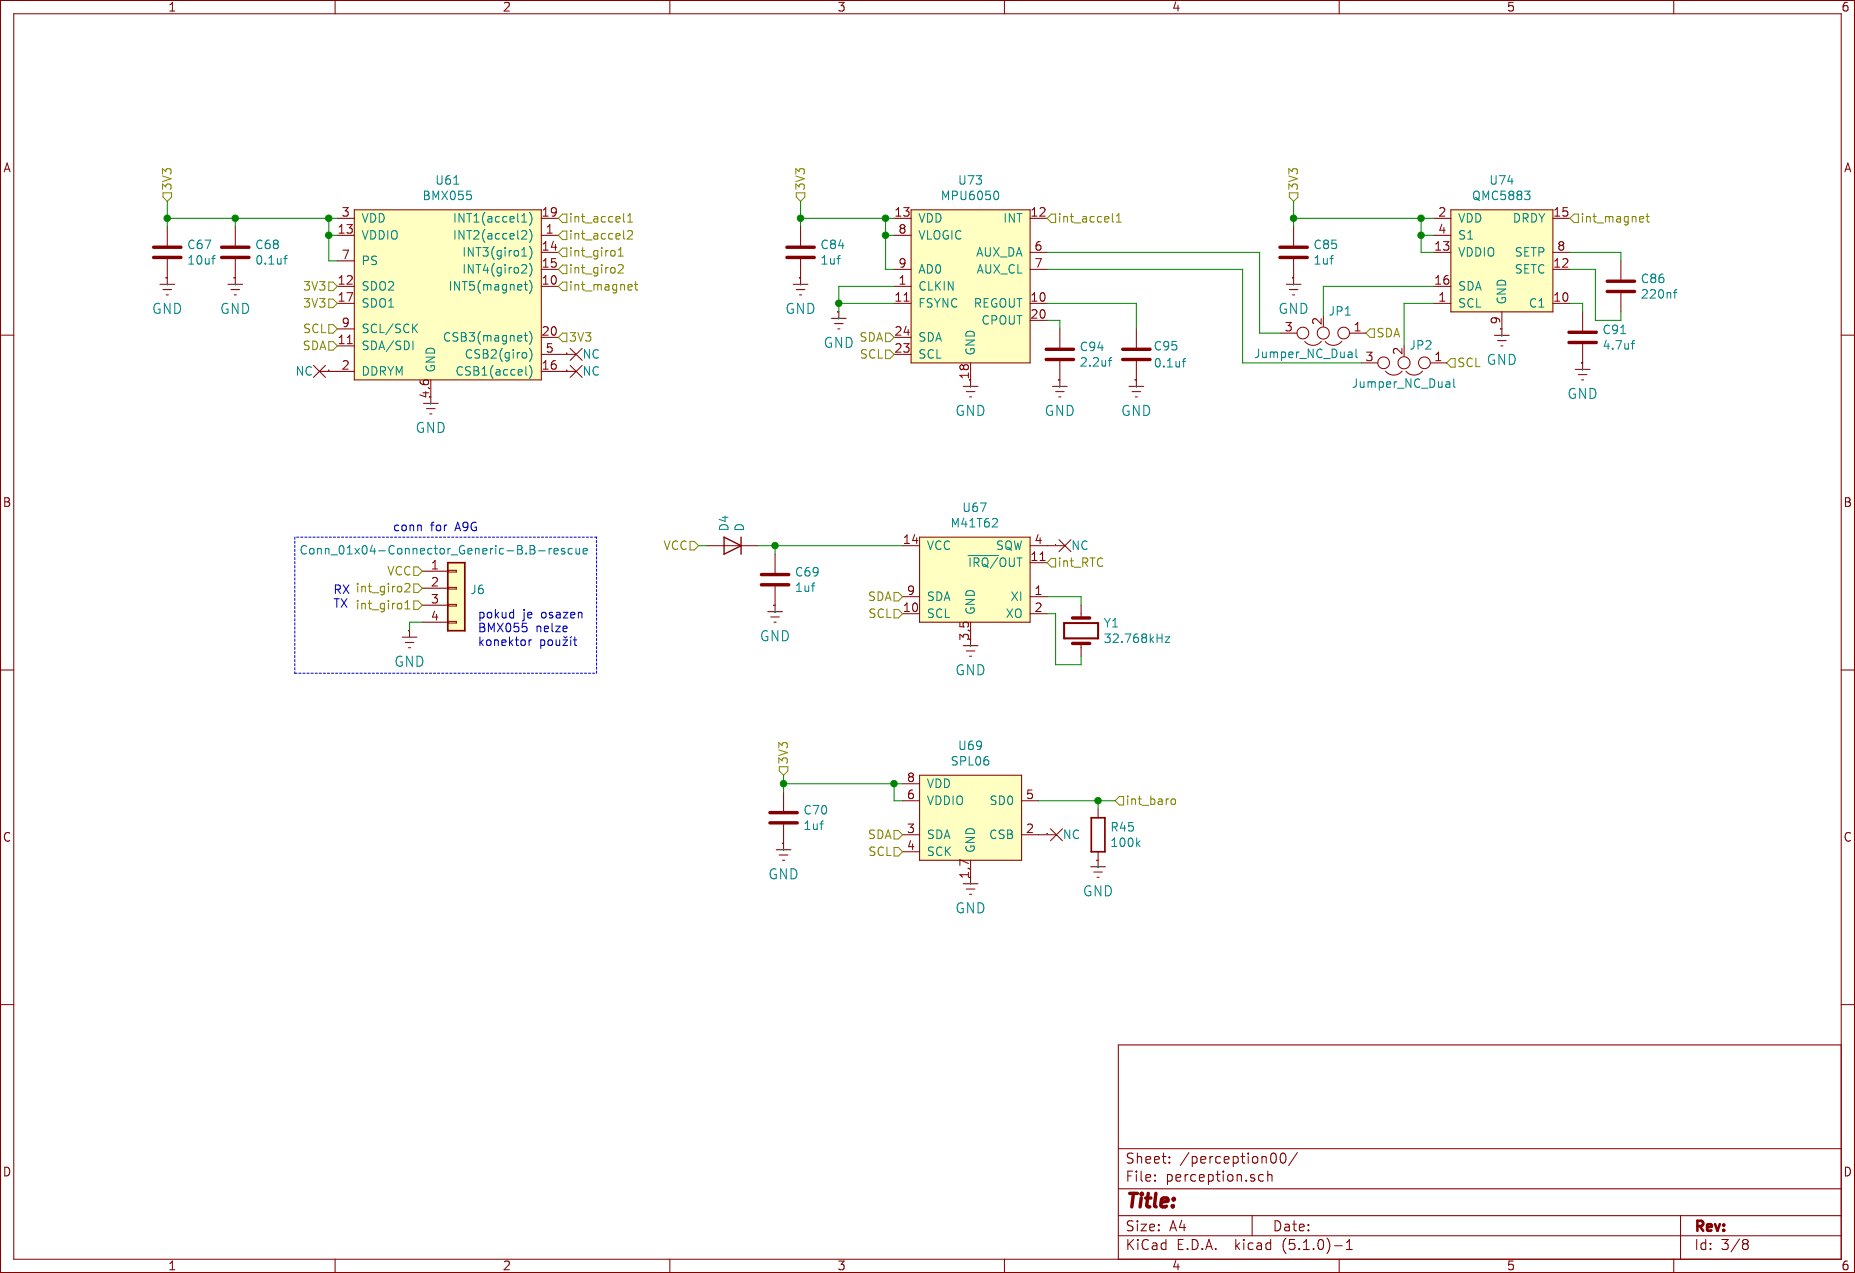
\includegraphics[width=0.93\textheight, angle=90]{kapitoly/ctvrta_elektronicka_varianta/E4_zapojeni/senzorika.png}
    \caption{Zapojení senzorů BMX055, MPU6050, QMC5883, M41T62, SPL06 a konektoru pro A9G -- schéma \centering}
    \label{fig:E4-sch_senzorika}
\end{figure}
\begin{figure}
    \centering
    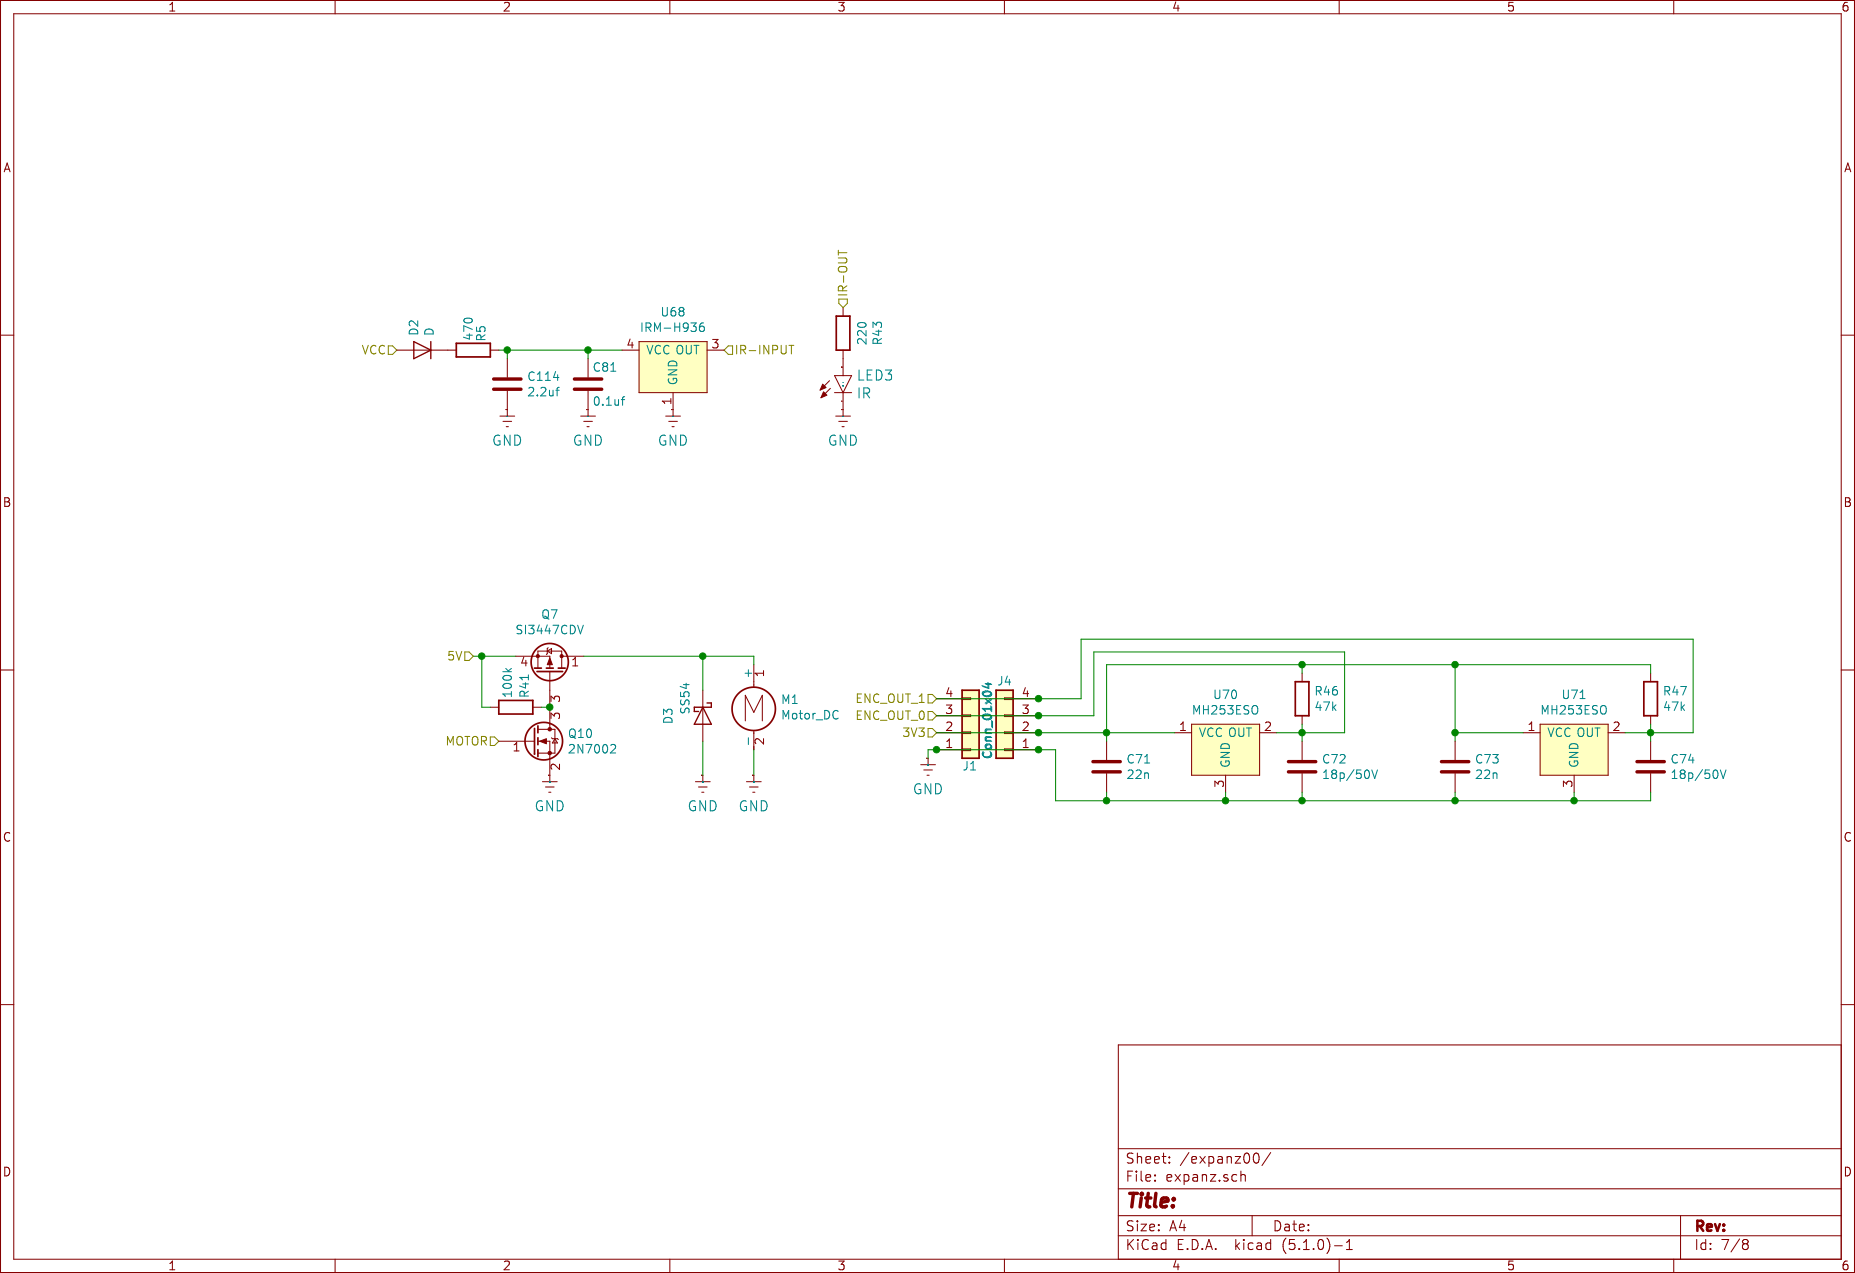
\includegraphics[width=0.93\textheight, angle=90]{kapitoly/ctvrta_elektronicka_varianta/E4_zapojeni/IR_motor_enkoder.png}
    \caption{Zapojení IR komunikace, motoru a enkodéru -- schéma}
    \label{fig:E4-sch_IR-Motor-enkoder}
\end{figure}
\begin{figure}
    \centering
    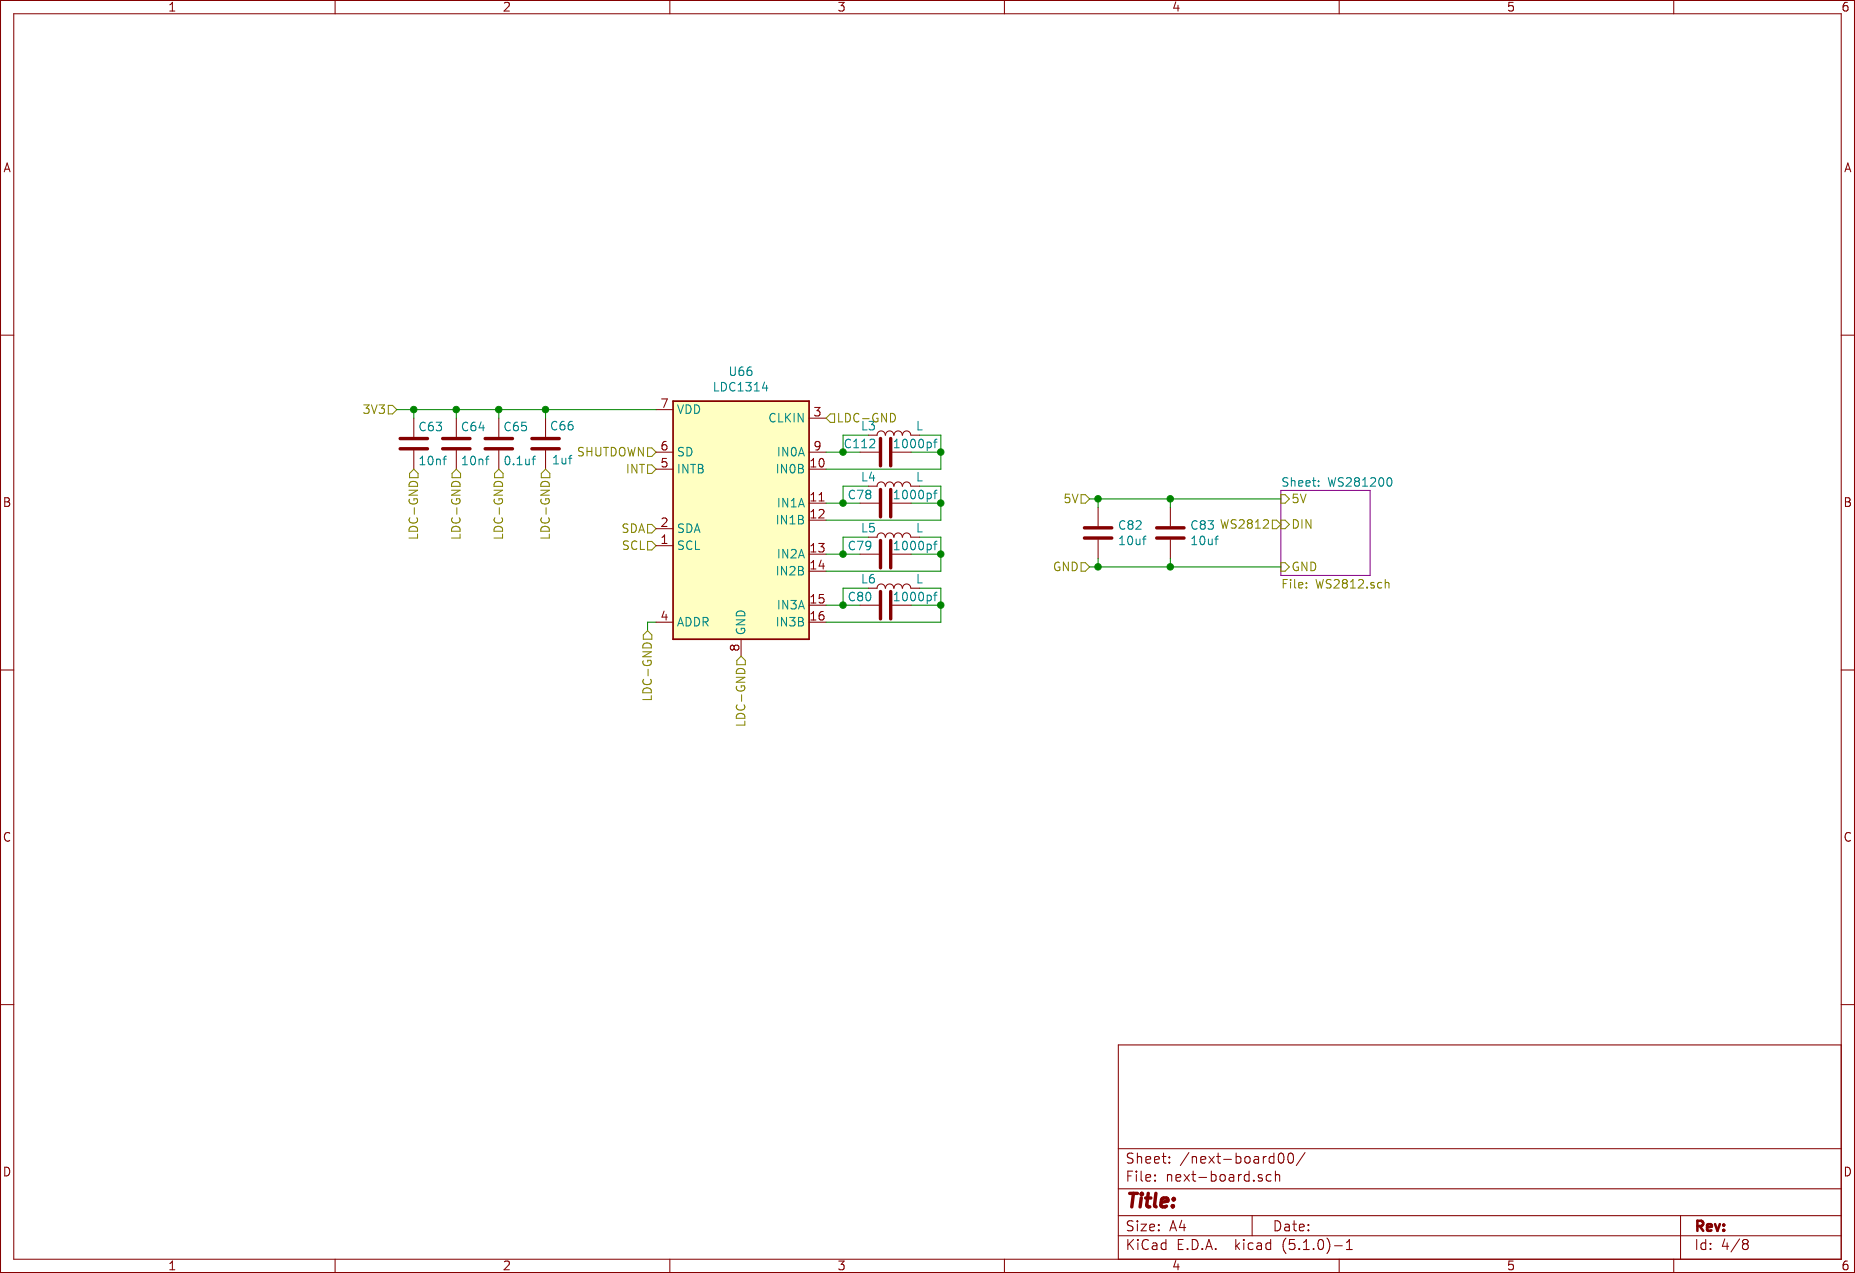
\includegraphics[width=0.93\textheight, angle=90]{kapitoly/ctvrta_elektronicka_varianta/E4_zapojeni/next_board.png}
    \caption{Zapojení LDC1614 -- schéma}
    \label{fig:E4-sch_next-board}
\end{figure}
\begin{figure}
    \centering
    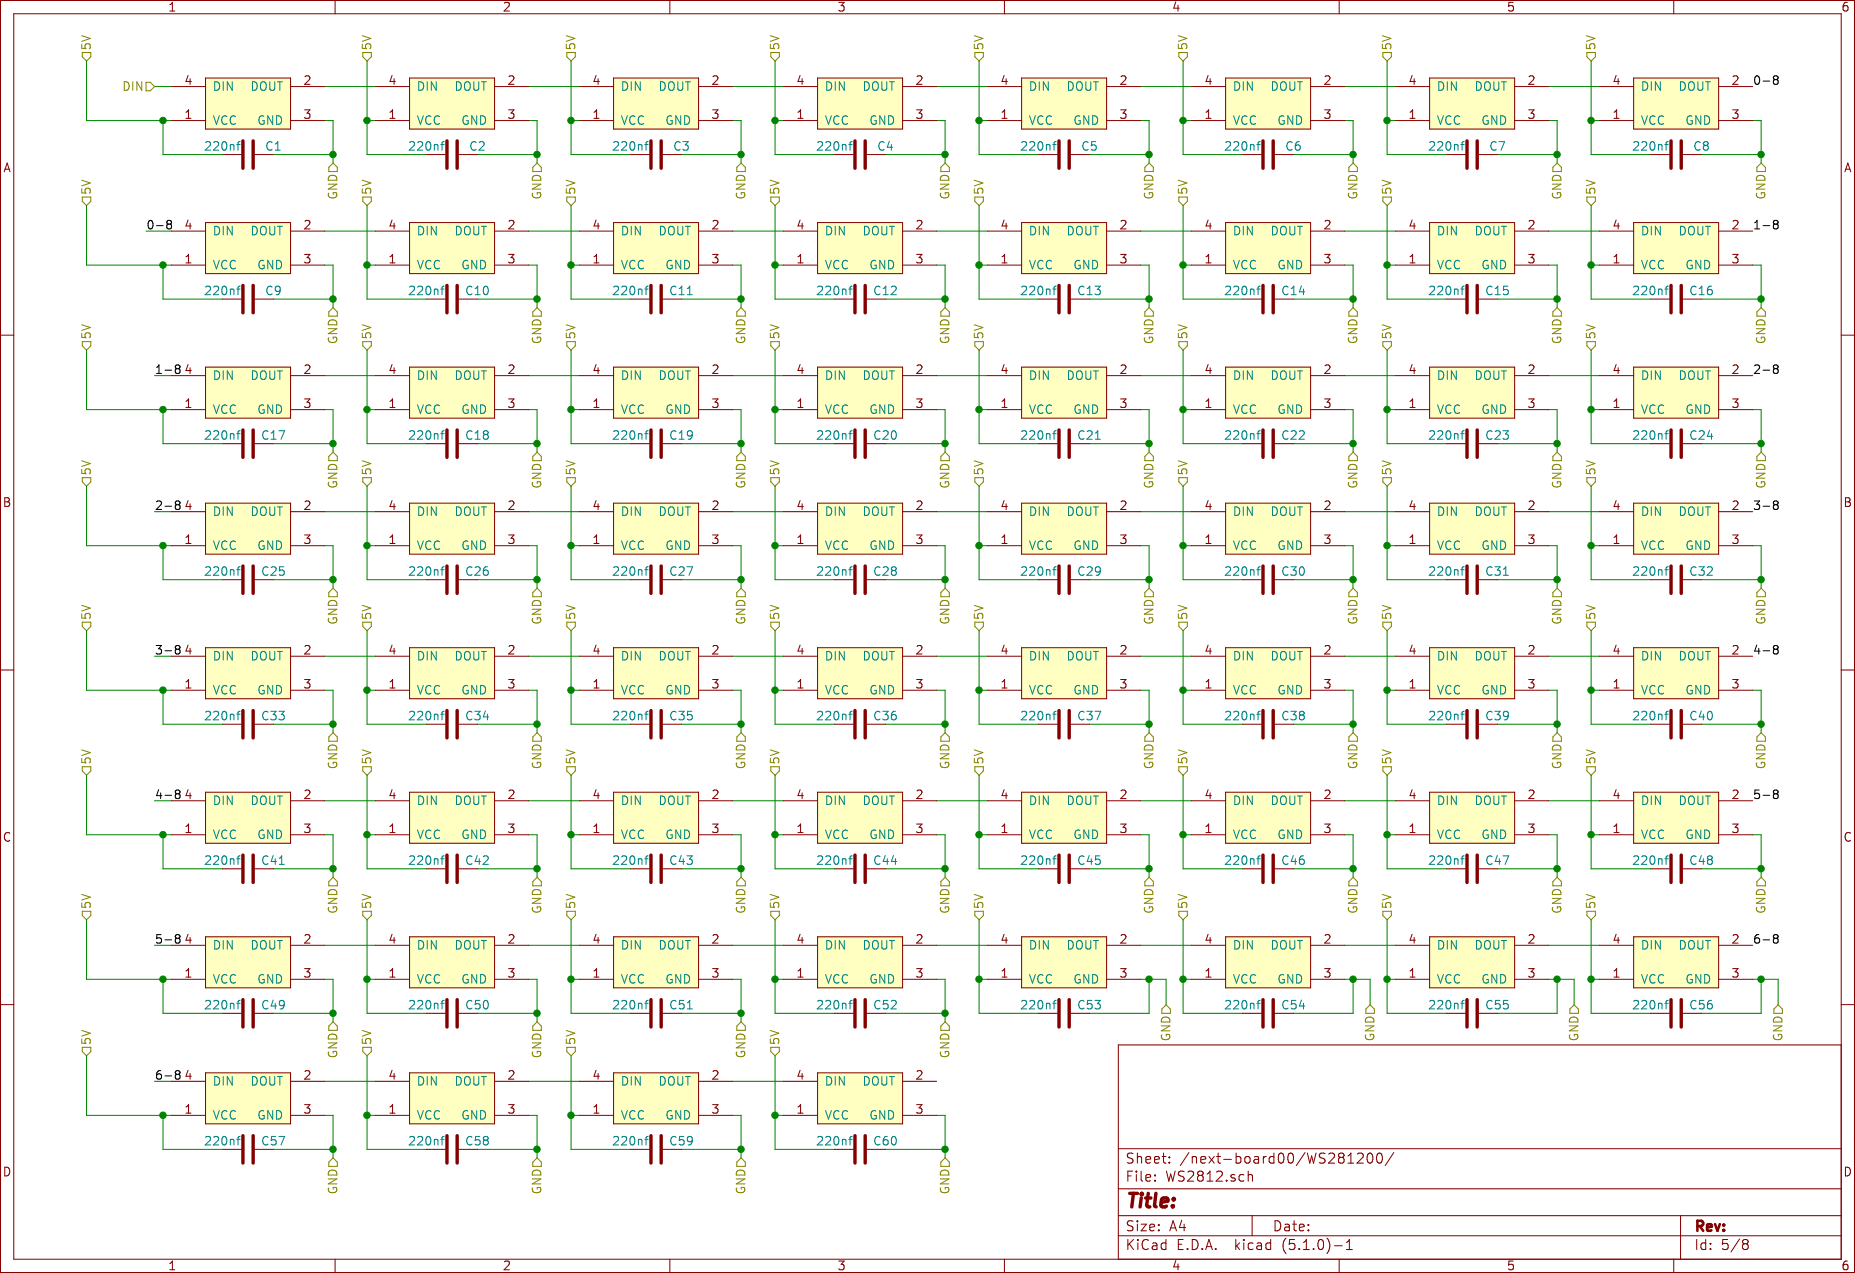
\includegraphics[width=0.93\textheight, angle=90]{kapitoly/ctvrta_elektronicka_varianta/E4_zapojeni/WS2812.png}
    \caption{Zapojení LED WS2812 na desce trezoru -- schéma}
    \label{fig:E4-sch_WS2812}
\end{figure}